\documentclass[12pt,a4paper,oneside]{report}
\usepackage[T1]{fontenc}
\usepackage[utf8]{inputenc}
\usepackage{lmodern,microtype}
\usepackage[margin=30mm,headheight=16pt]{geometry}
\usepackage{setspace,graphicx,booktabs,tabularx,array,amsmath,amssymb}
\usepackage{caption,float,longtable,xcolor,fancyhdr,listings}
\usepackage[numbers,sort&compress]{natbib}
\usepackage[hidelinks]{hyperref}
\usepackage{bookmark}
\graphicspath{{../figures/}}
\onehalfspacing
\setlength{\parindent}{1.5em}
\setlength{\parskip}{0.25em}
\setlength{\emergencystretch}{3em}
\pagestyle{fancy}\fancyhf{}\fancyhead[L]{\small\nouppercase{\leftmark}}\fancyhead[R]{\small Shelfwise}\fancyfoot[C]{\thepage}\renewcommand{\headrulewidth}{0.3pt}
\fancypagestyle{plain}{\fancyhf{}\fancyfoot[C]{\thepage}\renewcommand{\headrulewidth}{0pt}}
\captionsetup{font=small,labelfont=bf,skip=7pt}
\newcolumntype{Y}{>{\raggedright\arraybackslash}X}
\newcommand{\fig}[4][0.56]{\begin{figure}[H]\centering\includegraphics[width=\textwidth,height=#1\textheight,keepaspectratio]{#2}\caption{#3}\label{#4}\end{figure}}
\lstset{basicstyle=\ttfamily\footnotesize,backgroundcolor=\color{gray!7},frame=single,breaklines=true,columns=fullflexible,showstringspaces=false}
\hypersetup{pdftitle={Development of an Inventory and Stock Warning System for Small Supermarkets},pdfauthor={Author Name (Placeholder)}}
\begin{document}
\begin{titlepage}\centering
{\large UNIVERSITY NAME (PLACEHOLDER)\par}\vspace{0.4em}{\large Department / School Name (Placeholder)\par}
\vfill{\Large\bfseries MASTER'S THESIS\par}\vspace{1em}{\LARGE Development of an Inventory and Stock Warning System for Small Supermarkets\par}\vspace{2em}{\large Degree Title (Placeholder)\par}
\vfill\begin{tabular}{p{0.42\textwidth}p{0.42\textwidth}}Master's degree student & Author Name (Placeholder)\\[1em]Supervisor & Supervisor Name (Placeholder)\\\end{tabular}
\vfill{\large City (Placeholder) 2026\par}\end{titlepage}
\pagenumbering{roman}
\chapter*{WORK OVERVIEW}\addcontentsline{toc}{chapter}{WORK OVERVIEW}
\section*{Research purpose and objectives}
The purpose of this work is to design and develop a reproducible web-based inventory and stock-warning system for a small supermarket. The project focuses on three operational questions: how the current stock position is known, how every quantity change can be explained, and how staff can identify products that need attention before a shelf becomes empty.

The objectives are to analyse a single-store inventory domain; define a role and permission model; design a relational inventory ledger and warning lifecycle; implement a Spring Boot and Vue 3 application backed by MySQL and Redis; verify duplicate, concurrent, invalid, and failure scenarios; and prepare evidence suitable for a software-engineering thesis.
\section*{Technical contribution}
The implemented system combines four mechanisms in one auditable path: a product row lock for concurrent stock changes, actor-scoped idempotency keys for retries, persisted warning episodes that separate stock recovery from acknowledgement, and revision-keyed Redis caching that falls back to MySQL. The project presents these as engineering design decisions and verified behaviors rather than as new algorithms.
\section*{Submission and artifact requirements}
The deliverables are the runnable system, schema migration, API and deployment documentation, source diagrams, reproducibility scripts, evidence data, and this English thesis. The author, university, department, degree, supervisor, and student number remain placeholders because they were not supplied. No institutional compliance or real-store trial is claimed.
\section*{Personal contribution}
The implementation covers the domain analysis, API and database design, backend and frontend development, security configuration, integration tests, browser checks, performance measurement, failure testing, evidence capture, and thesis preparation. All reported measurements are from the repository's scripts and local validation environment.
\section*{Structure and scope of the thesis}
Chapter 1 introduces the supermarket inventory domain and the object of analysis. Chapter 2 defines the assignment, requirements, related systems, and technology choices. Chapter 3 designs the architecture, database, permissions, and security boundaries. Chapter 4 describes implementation, routing, core functions, versioning, and deployment. Chapter 5 reports functional, integration, browser, performance, and recovery tests. The conclusion answers the project questions and states the limitations.
\tableofcontents\listoffigures\listoftables\clearpage\pagenumbering{arabic}
\chapter{Object analysis}

\FloatBarrier

\section{Description of the subject area}

A supermarket inventory system relates identifiable products to the quantities available for store operations. Goods arrive through deliveries and leave through sales, transfers, damage and other dispatches, while physical counts produce observations that may disagree with the recorded balance. Even though Shelfwise neither executes sales nor places orders with suppliers, it must represent the stock effect of both. The subject of this thesis is this inventory workflow within a single store.


The current balance and the movement history answer different questions. The balance answers a short operational one—how much of this product is recorded now?—whereas the history answers a longer explanatory one: which accepted changes produced that balance? A system that keeps only the balance cannot recover an omitted reason or tell a double submission from two genuine deliveries. A system that keeps only events can explain every change but needs extra work to serve fast, filtered inventory pages. Shelfwise therefore stores the balance together with its accepted movement records.


Each product carries descriptive context: identity, category, supplier, unit and current price. The SKU is a required unique identifier and the barcode is optional. Stock received through a purchase may also carry a batch number, production date and expiry date. The unit label always describes a whole-number quantity, so a label such as kg does not add decimal weighing; a weighing workflow would require fractional units and an explicit rounding policy. Sellable quantity excludes expired and quarantined batches, whereas physical quantity still includes them for disposal and reconciliation.


Inventory value is a presentation estimate: the current physical quantity of each active product multiplied by its current unit price. It is neither supplier cost, historical cost of goods sold nor an accounting valuation, and keeping this distinction prevents a convenient dashboard figure from being read as financial evidence. Likewise, the store currency preference changes only the displayed currency code and symbol and does not convert stored prices.


\FloatBarrier

\section{Operational problems and system boundary}

Manual stock work fails in several distinct ways. A delivery may be entered twice after a slow response; two dispatches may each rely on an outdated balance; a correction may be entered as a relative change when the employee meant an absolute count; and a manager may acknowledge a warning while the item is still out of stock. Because these are different problems, their controls must preserve their meanings instead of reducing every case to a generic update.


The system boundary covers product and reference-data administration, searchable inventory, receiving, dispatch, adjustment, stocktake, batch control, expiry and slow-moving warnings, warning review, replenishment suggestions, purchase drafting and approval, partial receipts, count and disposal reviews, reports and staff access. It excludes payment processing, supplier invoicing, checkout integration, customer reservations and multiple stores. A supplier record remains purely descriptive until a purchase document refers to it, and a purchase document affects stock only once a receipt is accepted.


The case study uses fictitious supermarket records and a local deployment. Its evaluation covers transaction correctness, request authorization, warning behavior and selected performance and recovery scenarios; effects on shelf availability or employee productivity would require evaluation with store staff and operational data. Table~\ref{tab:scope} summarizes the resulting boundary.


\begin{table}[htbp]\centering\small\setstretch{1.05}\setlength{\tabcolsep}{3pt}\renewcommand{\arraystretch}{1.25}
\caption{Implemented domain and excluded extensions}\label{tab:scope}
\begin{tabular}{>{\raggedright\arraybackslash}p{0.3\textwidth}>{\raggedright\arraybackslash}p{0.3\textwidth}>{\raggedright\arraybackslash}p{0.3\textwidth}}
\toprule
\textbf{Aspect} & \textbf{Implemented meaning} & \textbf{Extension outside the current boundary} \\
\midrule
\leavevmode{}Store organization & \leavevmode{}One shared store workspace & \leavevmode{}Tenant and branch isolation \\
\leavevmode{}Quantity & \leavevmode{}Bounded integer balance & \leavevmode{}Decimal weights and unit conversion \\
\leavevmode{}Stock operation & \leavevmode{}Receive, dispatch, adjust and count, with batch-aware receipt and dispatch & \leavevmode{}Checkout and reserved stock \\
\leavevmode{}Supplier & \leavevmode{}Product partner, replenishment suggestion and purchase workflow & \leavevmode{}Invoices and settlement \\
\leavevmode{}Warning & \leavevmode{}Quantity, expiry, slow-moving and recovery episodes with review & \leavevmode{}Demand forecasting and automatic purchasing \\
\leavevmode{}Financial display & \leavevmode{}Current price multiplied by physical quantity as a presentation estimate & \leavevmode{}Accounting cost and profit \\
\leavevmode{}Phone access & \leavevmode{}Responsive browser interface & \leavevmode{}Native Android or iOS application \\
\bottomrule\end{tabular}\end{table}

\FloatBarrier

\section{Construction of the conceptual model}

The functional model in Figure~\ref{fig:functions} divides the system into seven modules: identity and access, catalog, stock activity, batches and reviews, warnings, purchasing and reporting. The modules carry different responsibilities but share the product identity. Catalog work defines what a product is and how it is classified; stock activity changes its bounded quantity; batches and reviews track dated stock and approve corrections; warnings interpret the quantity against policy and record review; purchasing turns shortages into approved orders and receipts; and reporting summarizes the accepted facts.


\begin{figure}[htbp]\centering
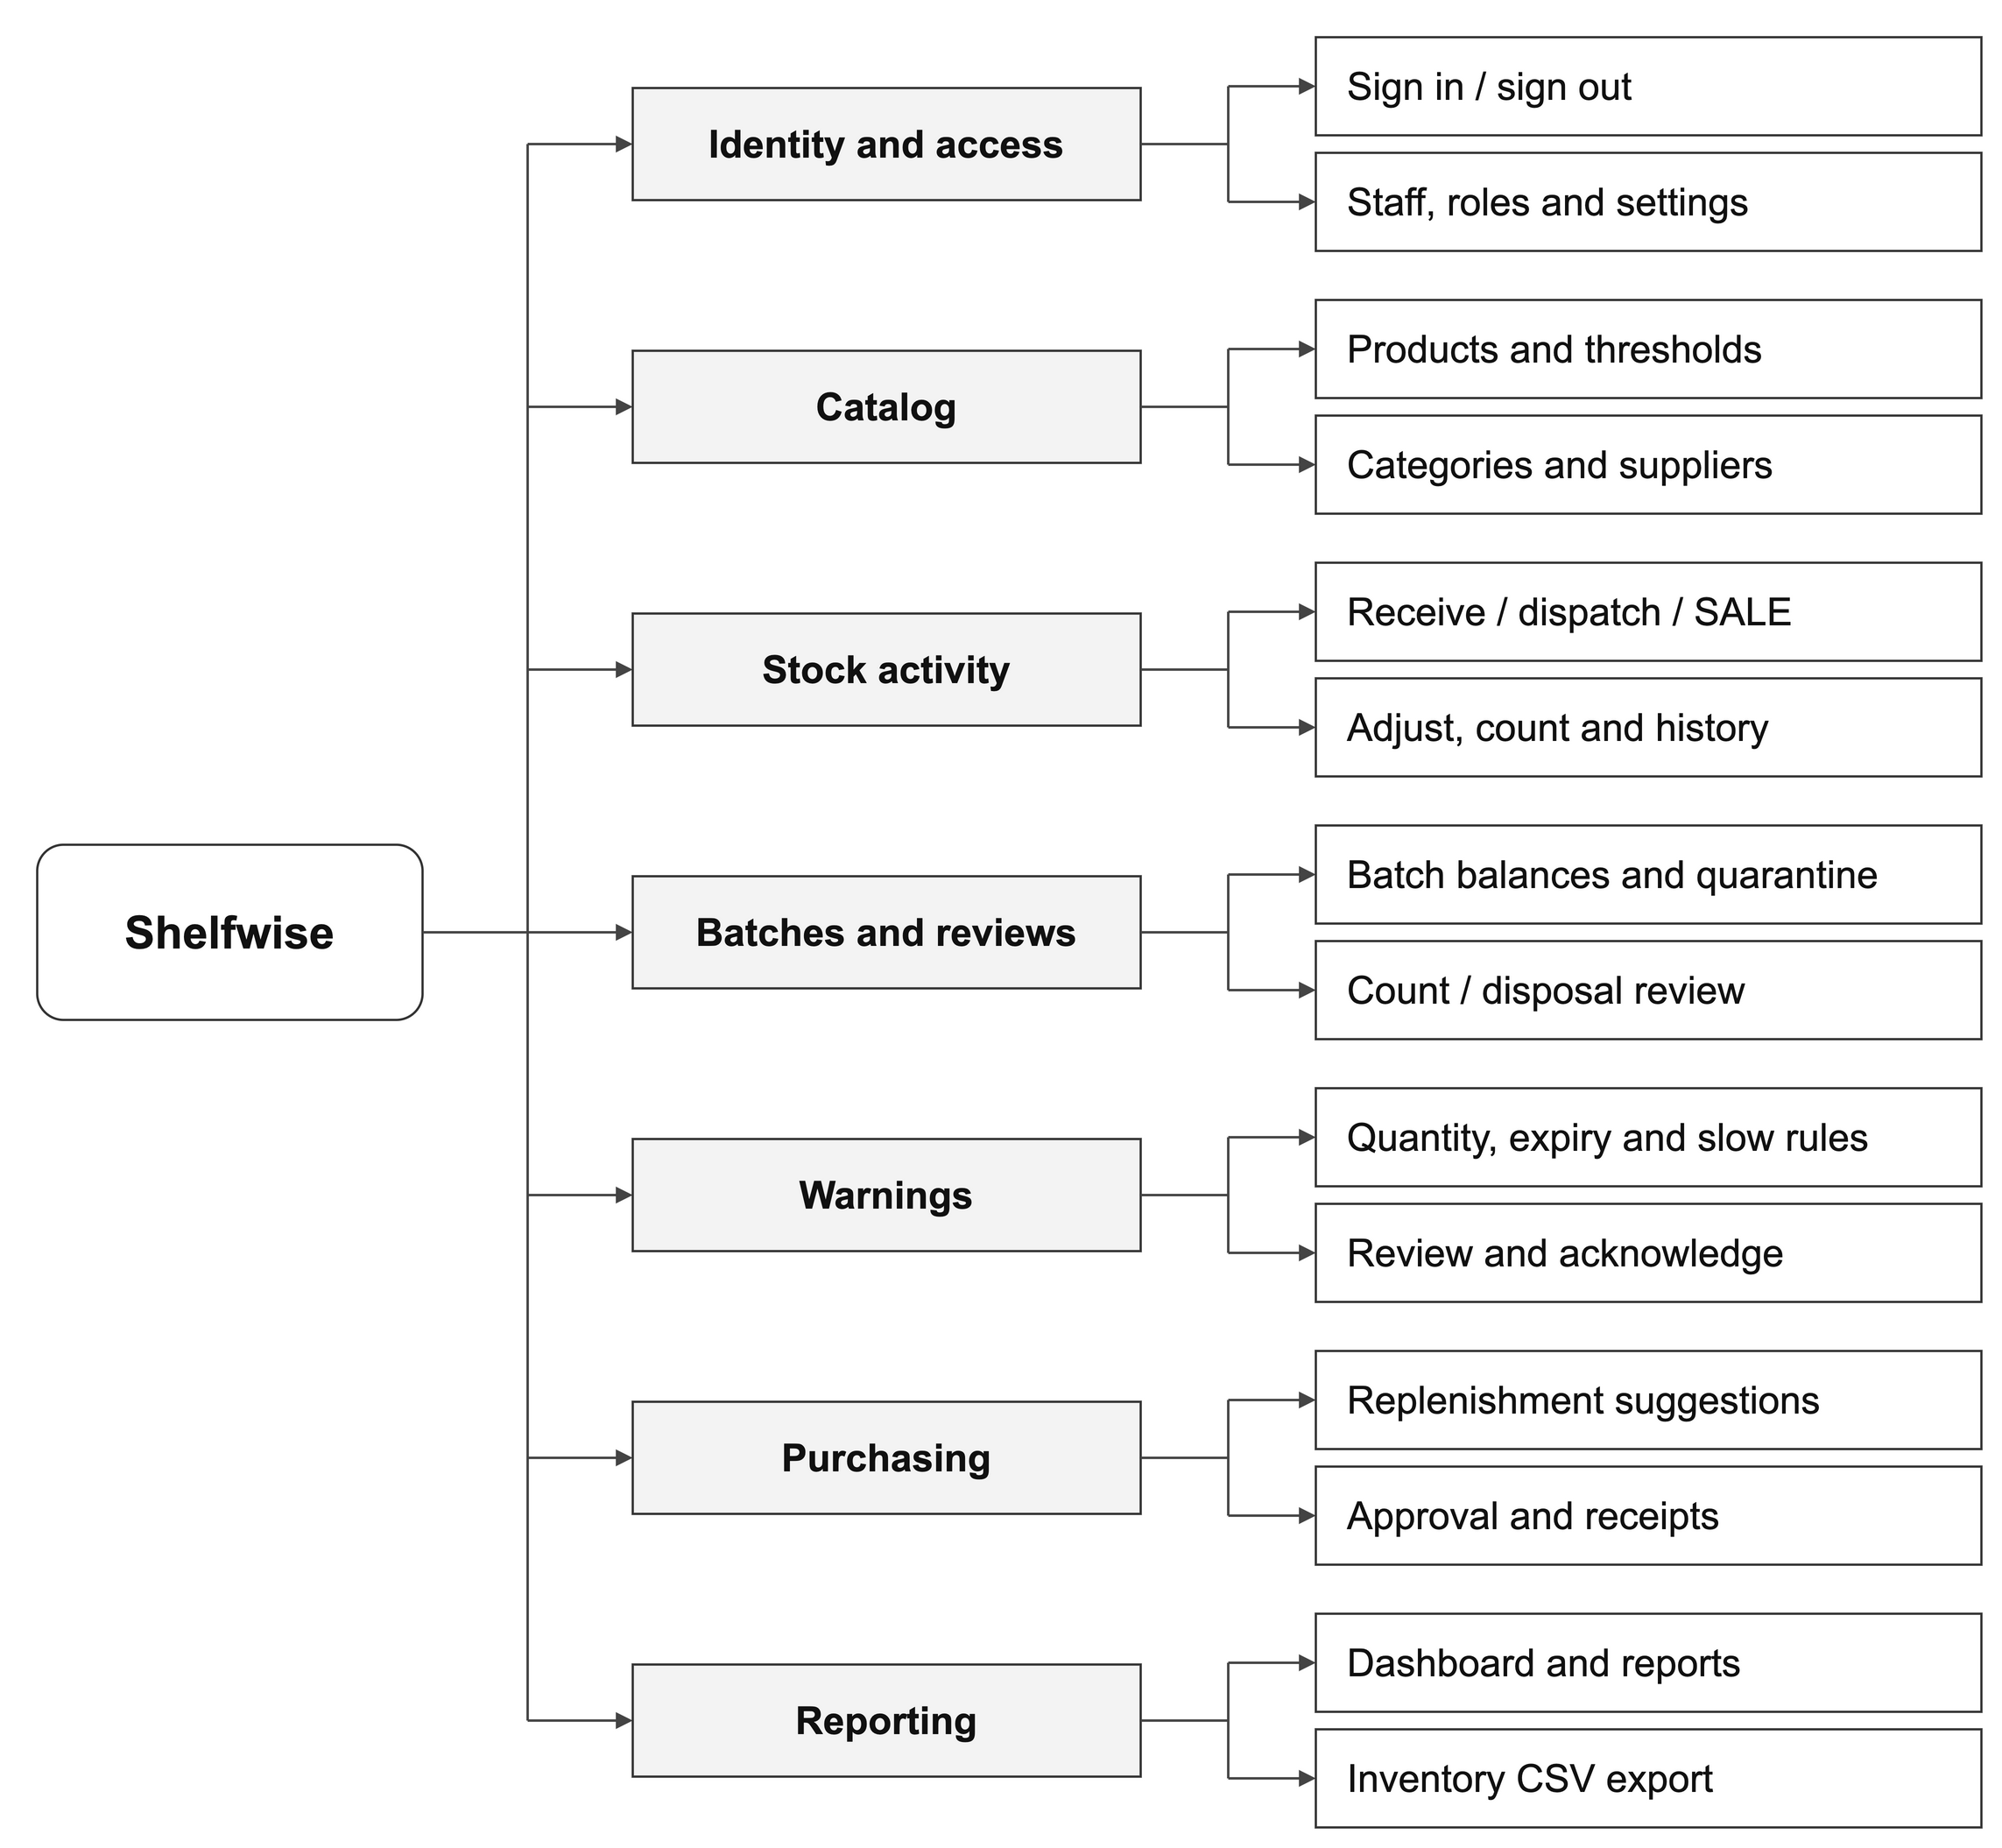
\includegraphics[width=\textwidth,height=0.70\textheight,keepaspectratio]{../figure-assets/diagrams/01-functional-model.png}
\caption{Overall functional model of the supermarket inventory system}\label{fig:functions}
\end{figure}

The division is most useful when a requirement spans several modules. Receiving stock, for example, changes a product, creates a movement, may resolve a shortage and alters dashboard totals. Separate responsibilities do not imply separate services, and Chapter 3 explains why these effects are coordinated within a single database transaction.


\subsection{Product catalog model}

A product has a SKU, an optional barcode, a name, a unit, a current price, a category and an optional supplier. Its stock policy consists of a safety stock and a reorder threshold. The current quantity is displayed alongside the product but cannot be entered in the catalog; it changes only through an inventory operation. An archived product keeps its identity and history but rejects further stock movements.


Authority over the catalog differs from authority over stock. Administrators manage product identity and archival, managers inspect inventory and update thresholds, and clerks consult product information before posting stock; the role matrix in Chapter 3 records the exact boundaries.


Categories organize the inventory view and its totals, and suppliers hold descriptive partner information that may be linked to products. Neither reference type owns a stock balance. Deleting a category or supplier that is still referenced violates its foreign-key relationship, so stock-bearing records follow the separate archival lifecycle instead.


\subsection{Stock activity model}

Shelfwise records five movement types, summarized in Table~\ref{tab:movements}. STOCK\_IN takes a positive quantity and increases stock. STOCK\_OUT and the manually recorded SALE also take positive quantities but decrease stock; only SALE counts as a sale for slow-moving detection, and it records the stock effect of a sale without any checkout or payment integration. ADJUSTMENT takes a signed, non-zero change. STOCKTAKE supplies an absolute observed quantity, from which the server derives the delta under the product lock. Every accepted record keeps the actual before quantity, the signed delta and the after quantity.


\begin{table}[htbp]\centering\small\setstretch{1.05}\setlength{\tabcolsep}{3pt}\renewcommand{\arraystretch}{1.25}
\caption{Meaning of stock input and resulting change}\label{tab:movements}
\begin{tabular}{>{\raggedright\arraybackslash}p{0.225\textwidth}>{\raggedright\arraybackslash}p{0.225\textwidth}>{\raggedright\arraybackslash}p{0.225\textwidth}>{\raggedright\arraybackslash}p{0.225\textwidth}}
\toprule
\textbf{Movement type} & \textbf{Meaning of entered quantity} & \textbf{Derived delta} & \textbf{Operational example} \\
\midrule
\leavevmode{}\allowbreak{}\path|STOCK_IN|\allowbreak{}\allowbreak{} & \leavevmode{}Positive amount received & \leavevmode{}Positive entered amount & \leavevmode{}Morning delivery \\
\leavevmode{}\allowbreak{}\path|STOCK_OUT|\allowbreak{}\allowbreak{} & \leavevmode{}Positive amount dispatched & \leavevmode{}Negative entered amount & \leavevmode{}Goods leaving the stockroom \\
\leavevmode{}SALE & \leavevmode{}Positive amount sold & \leavevmode{}Negative entered amount & \leavevmode{}Manually recorded sale without checkout \\
\leavevmode{}ADJUSTMENT & \leavevmode{}Signed correction & \leavevmode{}Entered signed amount & \leavevmode{}Two damaged units removed \\
\leavevmode{}STOCKTAKE & \leavevmode{}Absolute observed amount & \leavevmode{}Observed amount minus locked balance & \leavevmode{}Weekly physical count \\
\bottomrule\end{tabular}\end{table}

The use cases in Figure~\ref{fig:uc-stock} separate routine stock posting from reviewed corrections. Administrators and clerks receive goods, dispatch them and record SALE movements. Clerks submit adjustments, counts and disposals through the stock-review workflow, and administrators or managers approve them; administrators additionally retain direct ADJUSTMENT and STOCKTAKE access through the API. All three roles can inspect movement history, and the server, not the client, supplies the authenticated actor and the before and after quantities.


\begin{figure}[htbp]\centering
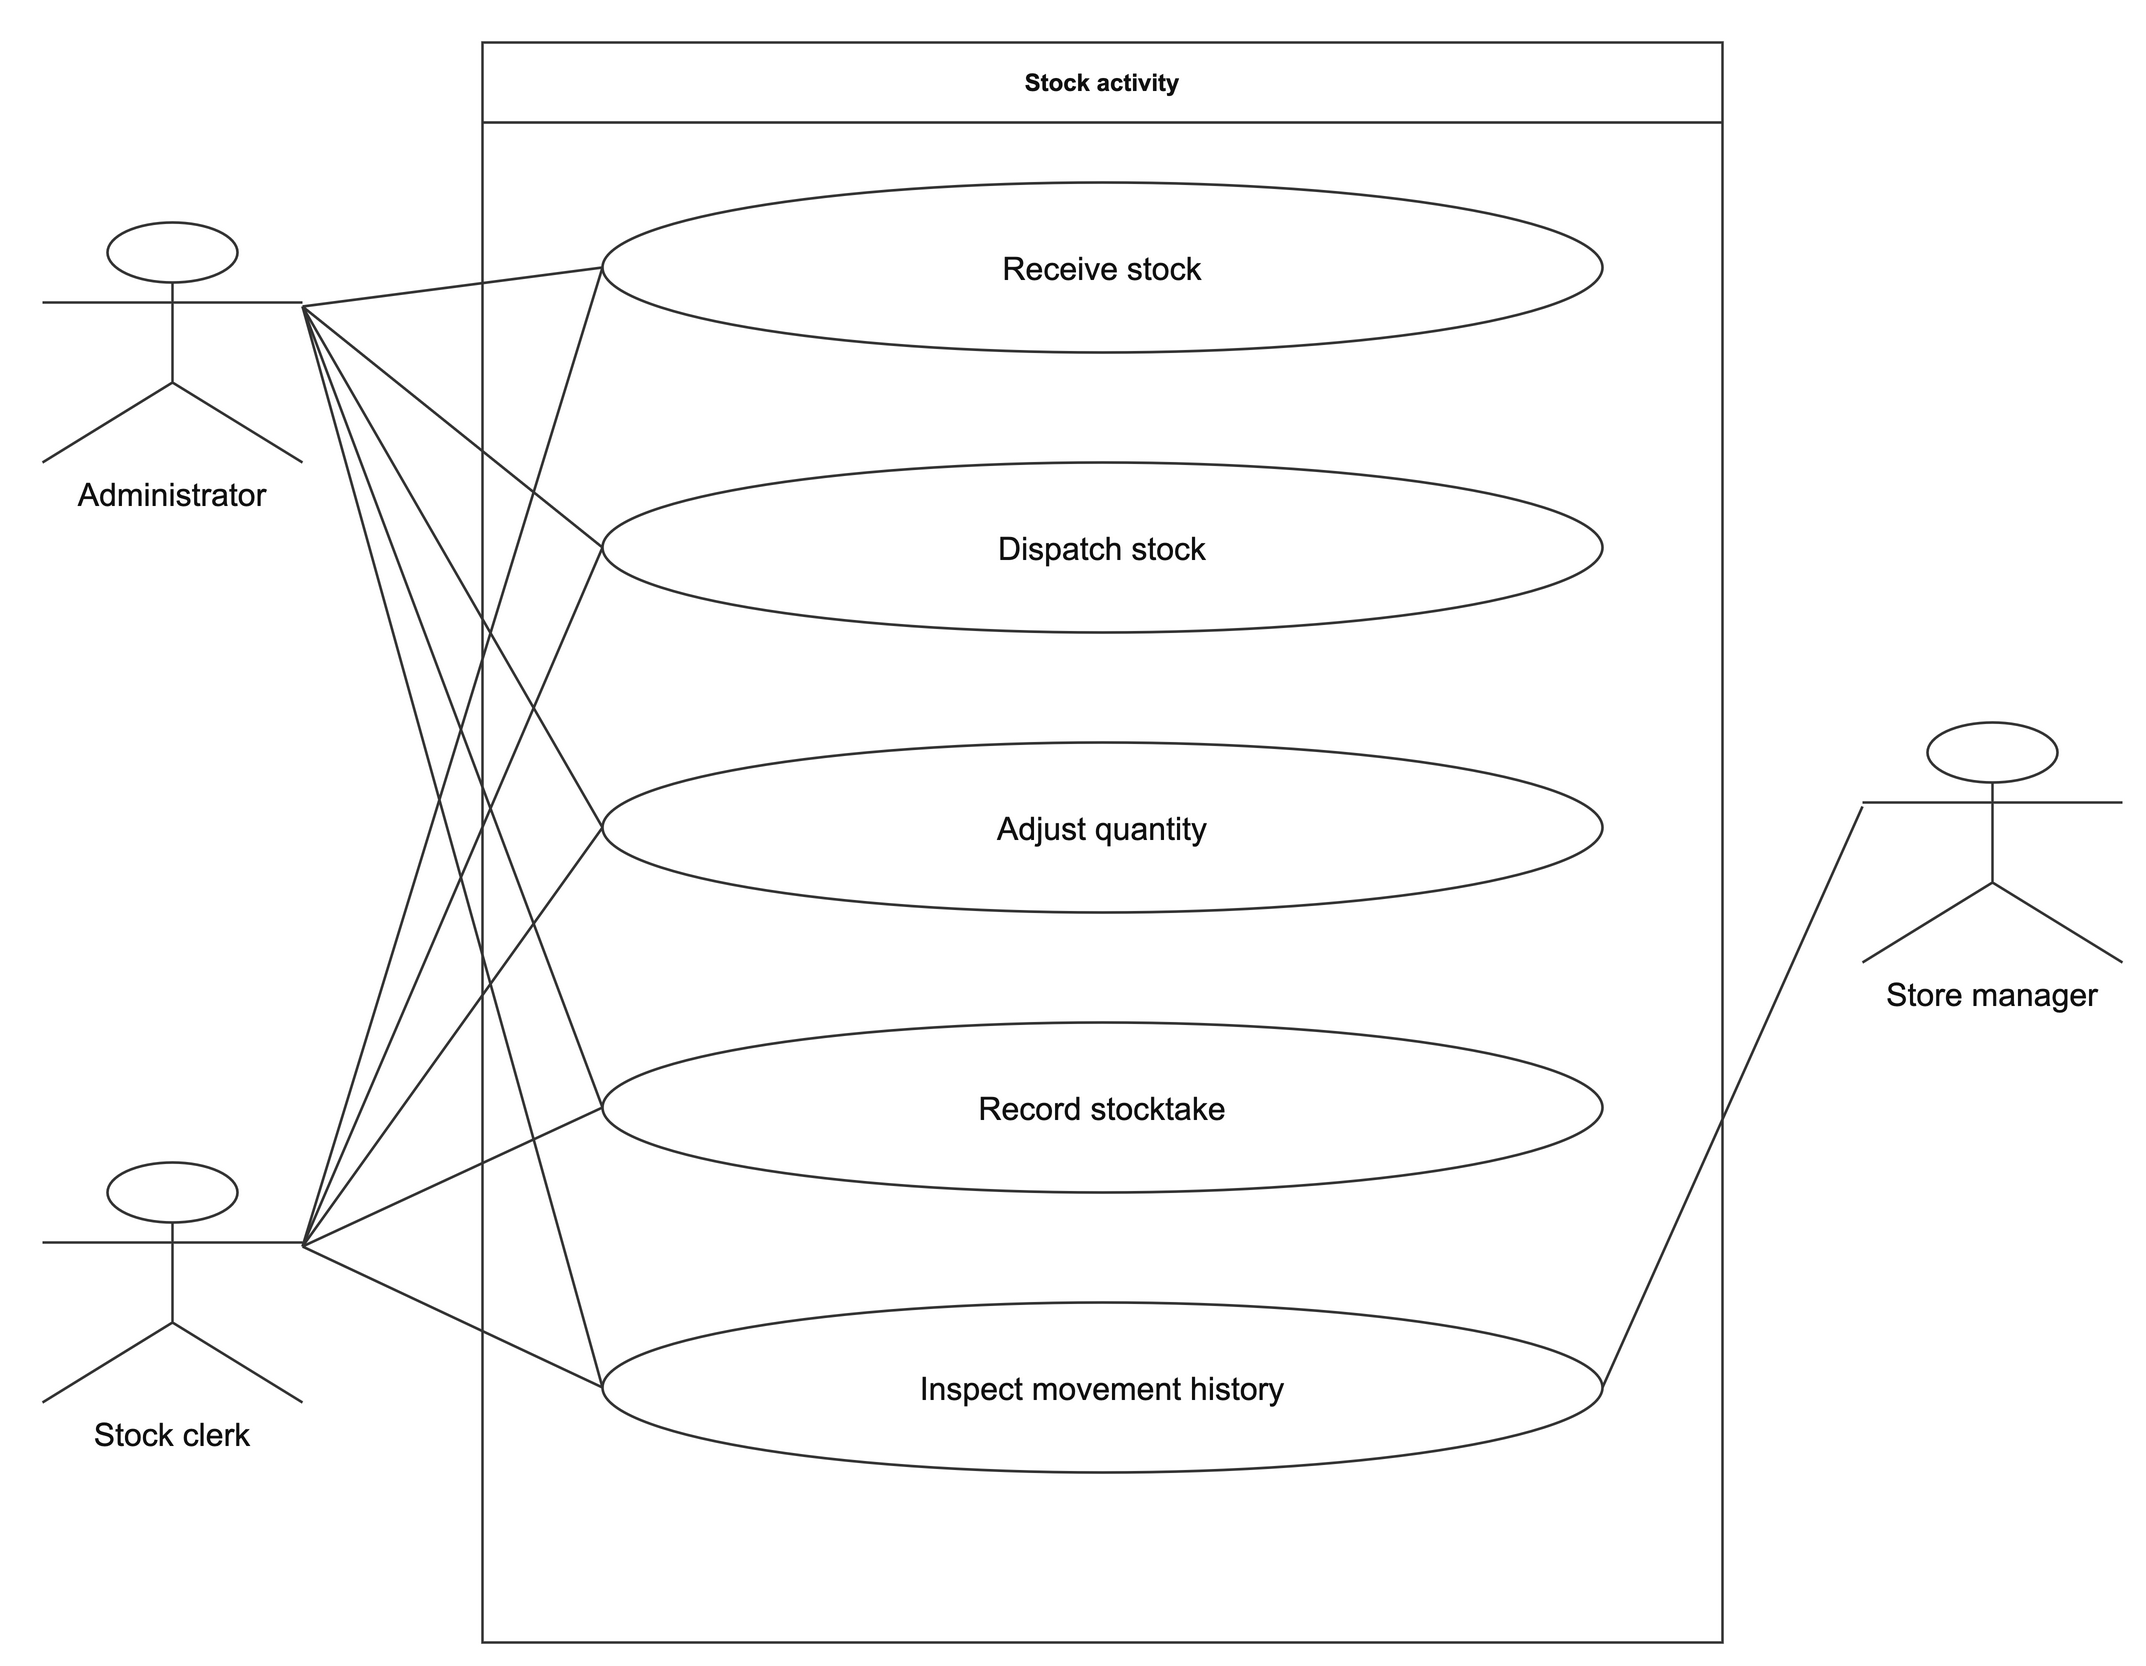
\includegraphics[width=\textwidth,height=0.70\textheight,keepaspectratio]{../figure-assets/diagrams/03-uc-stock.png}
\caption{Stock operation and history use cases}\label{fig:uc-stock}
\end{figure}

Every accepted movement carries a mandatory reason, an actor taken from authentication and a server-assigned timestamp, which together support the investigation of a disputed quantity. A correction is recorded as a further movement, so the earlier record is preserved.


\subsection{Warning and recovery model}

A warning is a persisted episode that links a product to a rule interpretation. OUT and LOW describe sellable quantity, EXPIRING and EXPIRED describe batch dates, SLOW describes a lack of sales over a configured window, and RESTOCKED records a recovery interval. Expiry dates are evaluated in the configured business timezone. A healthy replenishment can resolve a shortage and open a time-limited RESTOCKED episode, and acknowledgement remains independent of all these conditions.


Acknowledgement records a reviewer and a review time; it neither changes the quantity nor resolves the shortage. The distinction matters after a partial replenishment, when a reviewed product may still be LOW and the existing episode keeps its reviewer. A transition from LOW to OUT, or from OUT to LOW, resolves the old episode and opens a new one at the new severity.


Episodes serve both current attention and historical explanation. Open warnings tell a manager what currently needs review, and resolved records show when a shortage or recovery interval ended. The dashboard and warning board are views of these records rather than independent sources of stock truth. Figure~\ref{fig:warning-rules} shows the three rule families and the input each one reads: the quantity rule uses sellable quantity, the expiry rule uses batch dates and the slow-moving rule uses SALE movements only. All three write warning episodes, and none of them changes stock.


\begin{figure}[htbp]\centering
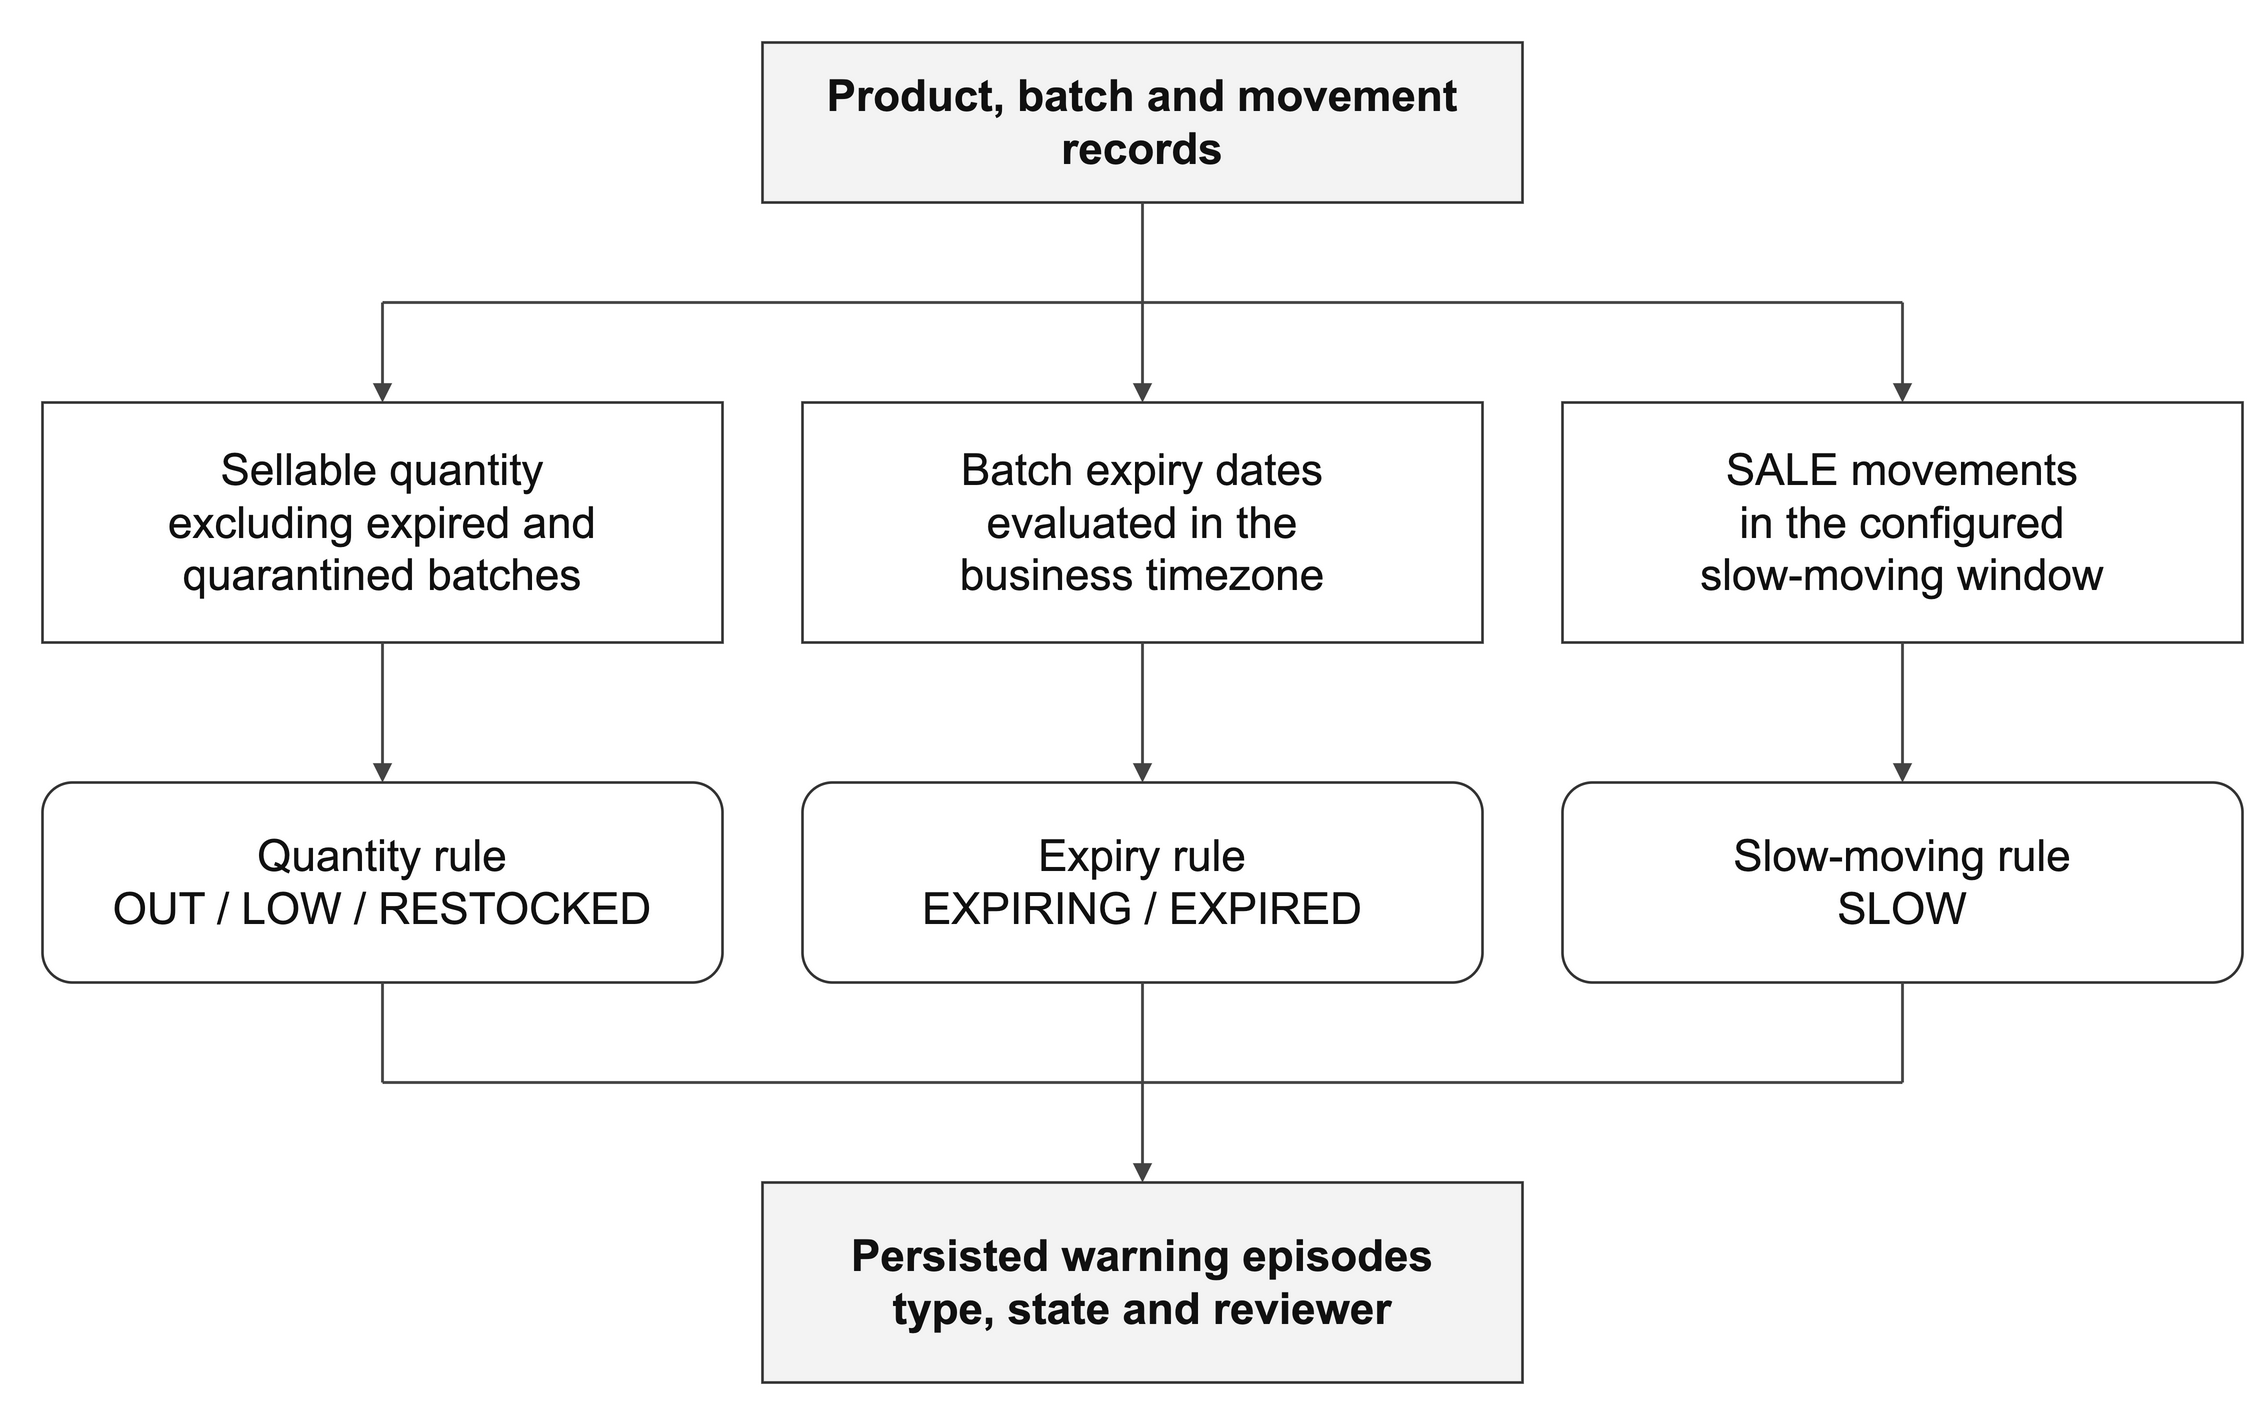
\includegraphics[width=\textwidth,height=0.70\textheight,keepaspectratio]{../figure-assets/diagrams/25-warning-rules.png}
\caption{Warning rule evaluation across batches, expiry, sales history and threshold policy}\label{fig:warning-rules}
\end{figure}

\subsection{Batch and purchasing objects}

A batch is the inventory identity created when a receipt carries production or expiry data, and physical and sellable quantities are maintained separately. FEFO selects the eligible batch with the earliest expiry date, and FIFO provides a deterministic order when dates are absent. Quarantine is an explicit control state that withdraws a batch from sale without erasing its movement history.


A replenishment suggestion compares sellable quantity plus the pending purchase position with the trigger threshold and target stock; it never creates an order on its own. A purchase document follows the states in Figure~\ref{fig:purchasing-workflow}. A draft is submitted and then approved or rejected; a rejected document can be edited back into a draft or resubmitted directly. Receipts against an approved document make it PARTIAL or COMPLETED, and any document that is not yet completed can be cancelled, which closes its remaining quantity. The document governs the internal purchasing decision and its inventory effects, while transmitting orders to suppliers remains outside the application.


\begin{figure}[htbp]\centering
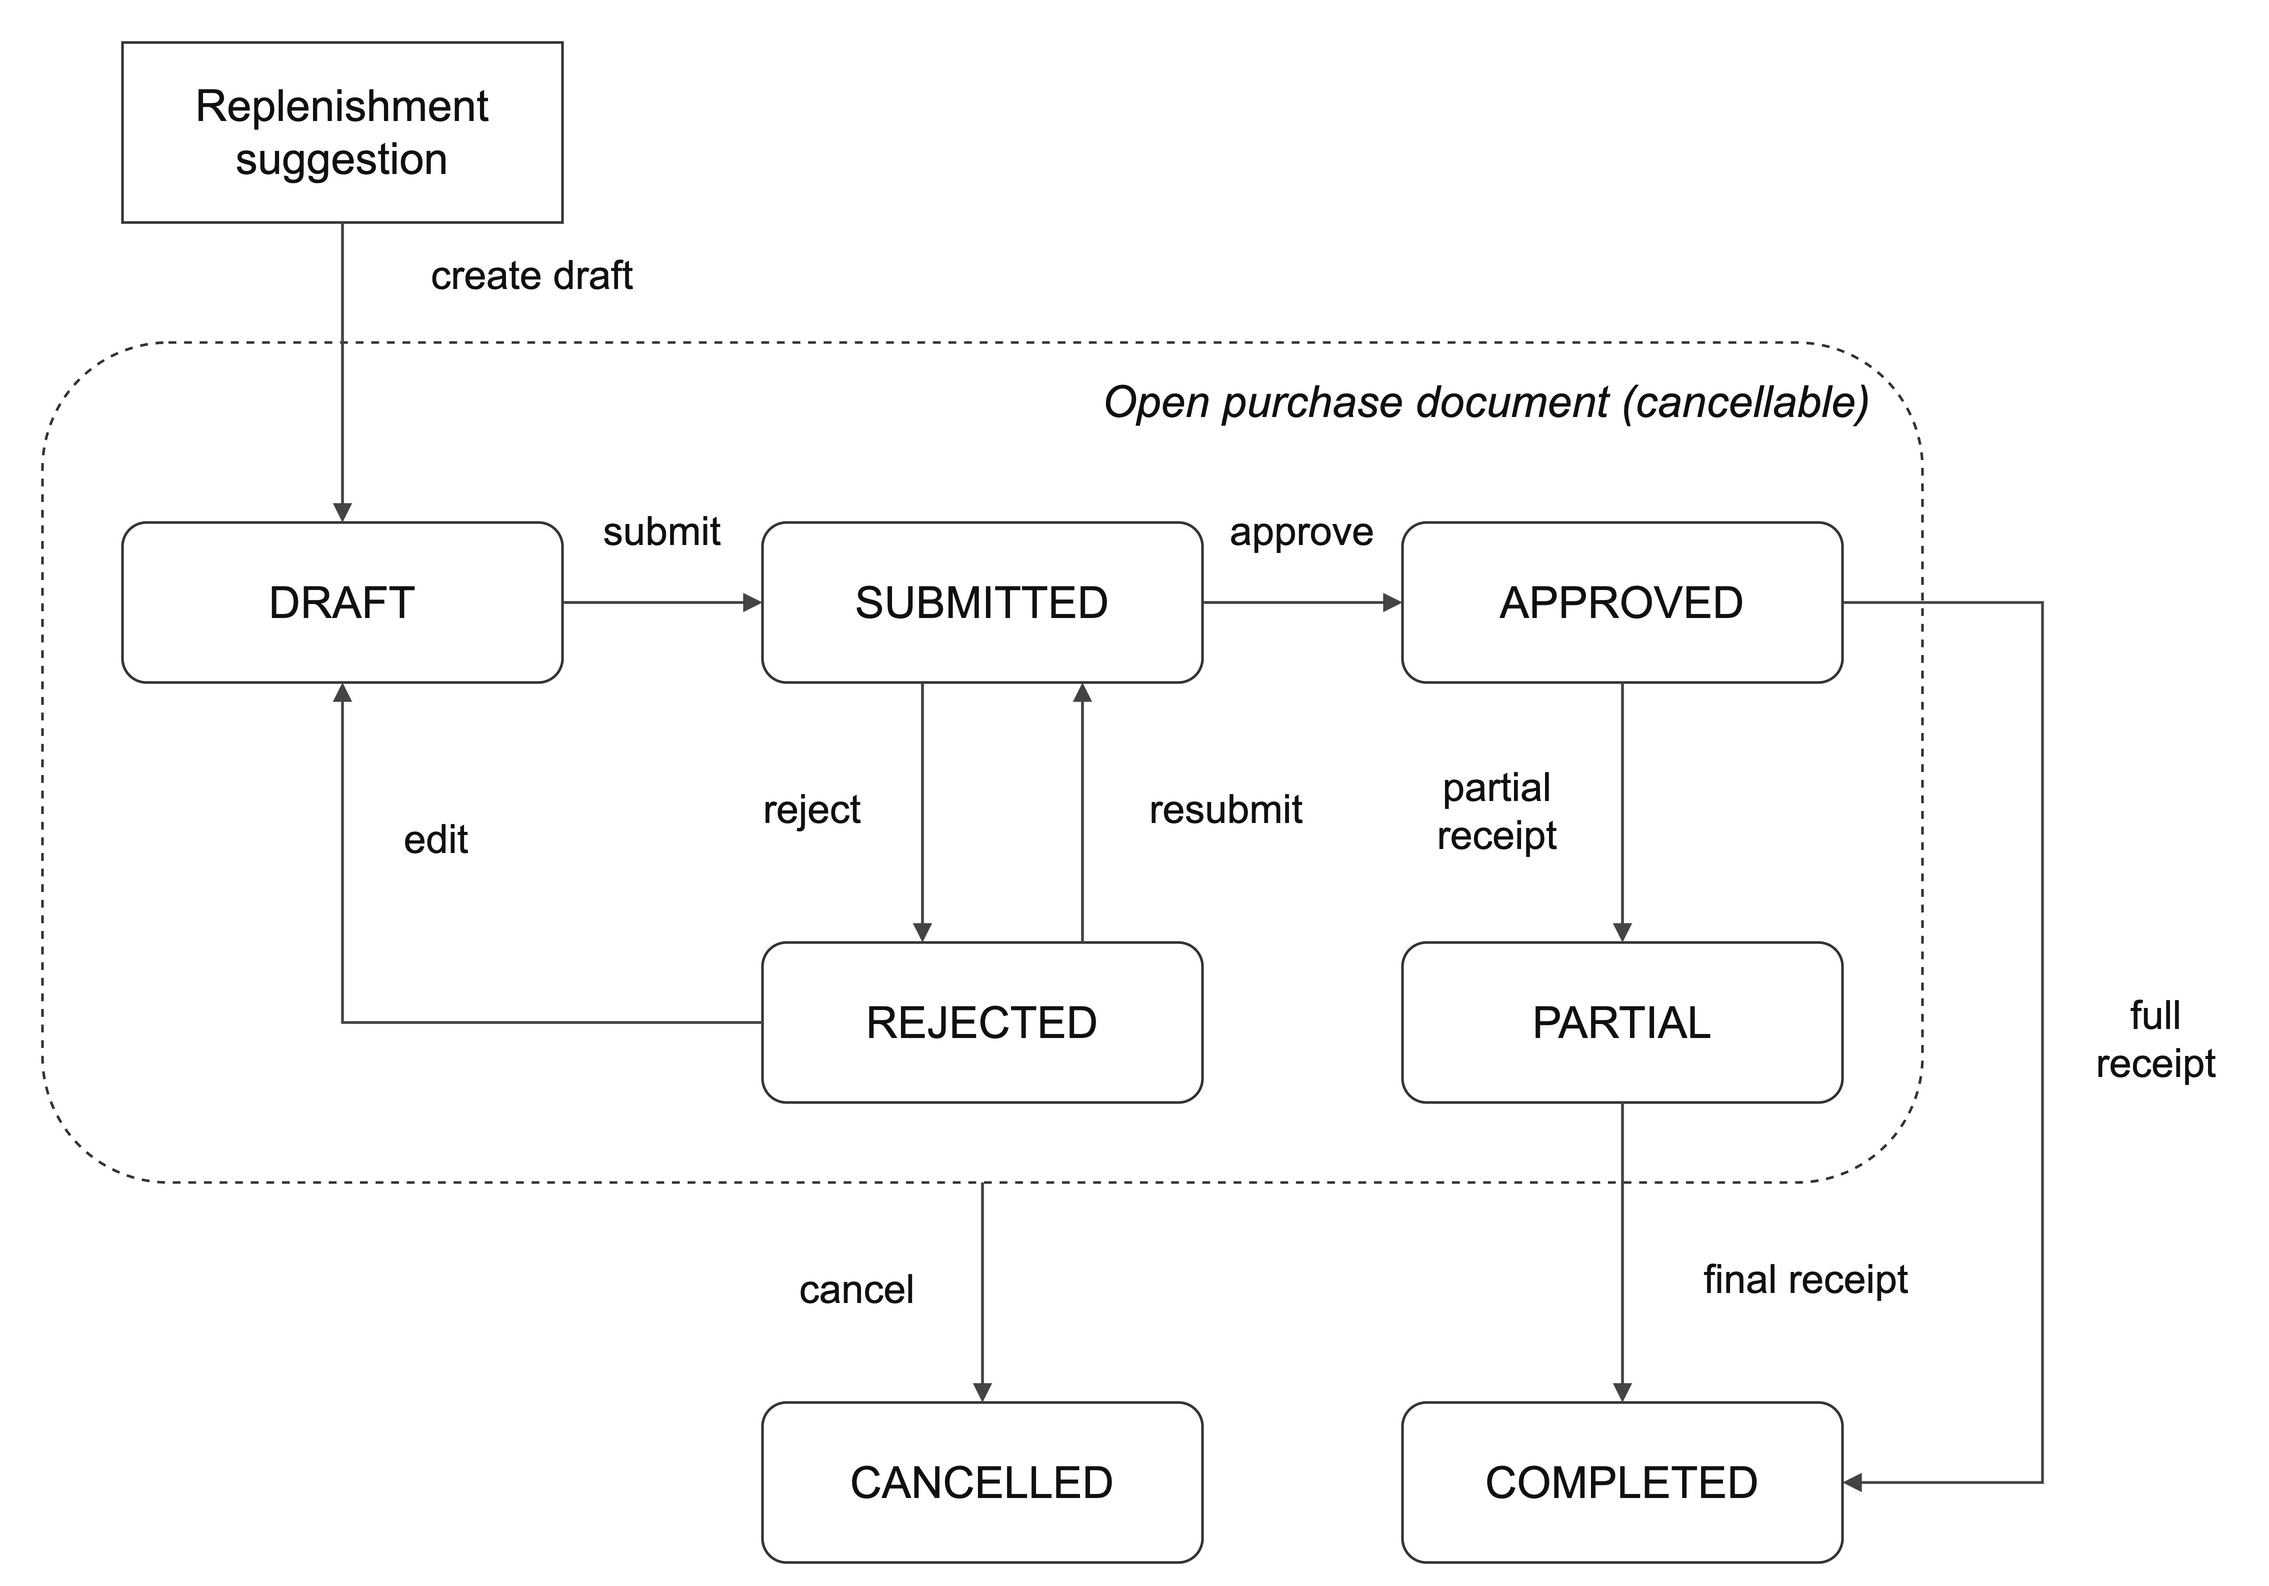
\includegraphics[width=\textwidth,height=0.70\textheight,keepaspectratio]{../figure-assets/diagrams/26-purchasing-workflow.png}
\caption{Replenishment suggestion through purchase approval and partial receipt}\label{fig:purchasing-workflow}
\end{figure}

A stock review records an intended count, adjustment or disposal against a quantity snapshot. Approval of a COUNT checks the product's quantity and version snapshot, approval of a DISPOSAL checks the remaining quantity of the selected batch, and an ADJUSTMENT applies its signed effect to the current locked balance. These checks prevent a delayed approval from overwriting a later receipt or dispatch.


\subsection{Reporting model}

Reports show active-product and shortage counts, the current-price value estimate, movement totals, recent activity and the category mix. The seven-day activity chart counts recorded movements by UTC date and is therefore not a sales chart, since receipts, adjustments and stocktakes also contribute. The category chart adds current unit counts, which is meaningful for the demonstration data but does not normalize different physical units.


The inventory CSV export contains the product page currently loaded. With twelve products per page, a large filtered selection may need several exports, each containing the fields visible on screen.


\subsection{Identity and administration model}

The application uses three fixed roles: ADMIN, MANAGER and CLERK. Each user has a username, display name, password hash, role, enabled flag and creation time. Administrators create users and change their access, while managers and clerks work within their assigned authority. Role changes and account suspension take effect on the next request, which limits reliance on authority cached in an old session.


At least one enabled administrator must always remain. This last-administrator guard prevents the store from losing access to staff administration. It complements rather than replaces authentication: a valid session still requires a currently enabled account whose role permits the requested action.


\FloatBarrier

\section{Domain invariants and representative scenarios}

The stock invariant combines arithmetic, bounds and attribution. The accepted after quantity equals the locked before quantity plus the derived delta, the balance and the movement record are written in the same transaction, and the quantity stays between zero and one billion. Product policy further requires a non-negative safety stock no greater than the reorder threshold. An invalid operation must leave both the balance and the history unchanged.


\begin{equation}q_{\mathrm{after}}=q_{\mathrm{before}}+\Delta,\qquad 0\leq q_{\mathrm{after}}\leq 10^9.\end{equation}

Consider a product with quantity seven and a reorder threshold of five. Dispatching two units leaves five and opens a LOW episode, because the threshold is inclusive. Dispatching the remaining five changes the severity to OUT. Acknowledging that episode records the review but leaves the quantity at zero. A later receipt of eight resolves the shortage and opens RESTOCKED. A subsequent count of three then yields a delta of minus five against the locked quantity of eight; it is not interpreted as adding three.


A retry is handled differently. Once an actor has recorded the count of three under a given key, resending the same normalized intention returns the earlier record, whereas a count of four under that key is rejected as a conflict. The rule of one intention per key thus links the business operation to the concurrency and retry design developed in Chapter 3.


\FloatBarrier

\section{Chapter summary}

The analysis identifies product balances, accepted movement history and warning episodes as the core consistency concepts, extended by batches, purchase documents and review snapshots. Chapter 2 turns these concepts into testable requirements.

\chapter{Requirements and technology selection}

\FloatBarrier

\section{Assignment and acceptance approach}

The assignment is to implement the inventory workflow of Chapter 1 as an inspectable single-store application. A requirement counts as complete only when its actor, server operation, data effect and acceptance evidence can all be identified. For the approval workflows added in the expanded release, the behavior on replay, on a stale snapshot and across state changes must also be defined. A screen that appears to offer an operation is insufficient if the matching server permission or transactional behavior is missing, and a correct API is equally insufficient if the interface presents an absolute count as a relative change.


The requirements in Table~\ref{tab:requirements} are grouped into identity, catalog, stock operations, inventory inspection, warning review, reporting and administration. Correctness concerns cut across these groups: retry handling belongs to stock operations but depends on the request key kept by the browser, and cache fallback belongs to warning retrieval but depends on the database remaining the durable owner. The table therefore also serves as a map across the implementation layers.


\begingroup\small\setstretch{1.05}\setlength{\tabcolsep}{3pt}\renewcommand{\arraystretch}{1.25}
\begin{longtable}{>{\raggedright\arraybackslash}p{0.3\textwidth}>{\raggedright\arraybackslash}p{0.3\textwidth}>{\raggedright\arraybackslash}p{0.3\textwidth}}
\caption{Functional requirements and acceptance evidence}\label{tab:requirements}\\
\toprule
\textbf{ID} & \textbf{Required behavior} & \textbf{Principal acceptance evidence} \\
\midrule\endfirsthead
\toprule
\textbf{ID} & \textbf{Required behavior} & \textbf{Principal acceptance evidence} \\
\midrule\endhead
\bottomrule\endfoot
\leavevmode{}R1 & \leavevmode{}Sign in and sign out with current role authority & \leavevmode{}Anonymous denial, invalid credentials, session and role checks \\
\leavevmode{}R2 & \leavevmode{}Maintain catalog categories and suppliers & \leavevmode{}Uniqueness validation, referenced-record conflicts and archival \\
\leavevmode{}R3 & \leavevmode{}Receive and dispatch stock with an audit record & \leavevmode{}Before–delta–after arithmetic and attributed history \\
\leavevmode{}R4 & \leavevmode{}Apply signed adjustments and absolute counts & \leavevmode{}Negative correction, count-to-zero and unchanged-count cases \\
\leavevmode{}R5 & \leavevmode{}Search, filter and paginate inventory & \leavevmode{}Empty result, stable ordering and page-size boundary \\
\leavevmode{}R6 & \leavevmode{}Maintain shortage and recovery episodes & \leavevmode{}Zero, equality, severity change, recovery and expiry scenarios \\
\leavevmode{}R7 & \leavevmode{}Record managerial acknowledgement independently & \leavevmode{}Reviewer visibility and unchanged stock quantity \\
\leavevmode{}R8 & \leavevmode{}Present stock reports and selected-page export & \leavevmode{}Server aggregates, rendered reports and export scope \\
\leavevmode{}R9 & \leavevmode{}Manage users, roles and store preferences & \leavevmode{}Administrator boundary, next-request access and last-admin guard \\
\leavevmode{}R10 & \leavevmode{}Resist duplicate and concurrent stock submission & \leavevmode{}Exact replay, changed-payload conflict and concurrent tests \\
\leavevmode{}R11 & \leavevmode{}Preserve warning results without Redis & \leavevmode{}Cache bypass comparison and recorded outage equivalence \\
\leavevmode{}R12 & \leavevmode{}Track batch balances and apply FEFO/\allowbreak{}FIFO allocation & \leavevmode{}Receipt replay, expiry boundaries and batch dispatch tests \\
\leavevmode{}R13 & \leavevmode{}Detect expiry and slow-moving conditions & \leavevmode{}Business-timezone and sales-only warning tests \\
\leavevmode{}R14 & \leavevmode{}Manage replenishment and purchase approval & \leavevmode{}Suggestion quantities, approval recheck, partial receipt and cancellation tests \\
\leavevmode{}R15 & \leavevmode{}Review counts and disposal with a snapshot & \leavevmode{}Stale snapshot, approval and idempotent review tests \\
\end{longtable}\endgroup

\FloatBarrier

\section{Functional requirements}

\subsection{Authentication and role-specific access}

Users must authenticate before they can read inventory, and the server exposes the current account and role through a session-based API. Administrators manage accounts, catalog records and preferences; managers review stock health, read reports and update thresholds; clerks record movements and inspect inventory history. These are fixed role bundles rather than a configurable permission hierarchy, following the separation of roles and permissions described in the RBAC literature \citep{sandhu1996}.


Figure~\ref{fig:permissions} shows the three bundles; the administrator holds every manager and clerk permission and adds product identity, staff accounts, store settings and direct corrections. Every protected operation must be authorized by the server: navigation guards spare users misleading paths, but a caller who bypasses the browser must receive the same decision. An account disabled after sign-in must not remain usable merely because its cookie still exists, and role changes must take effect on the next request.


\begin{figure}[htbp]\centering
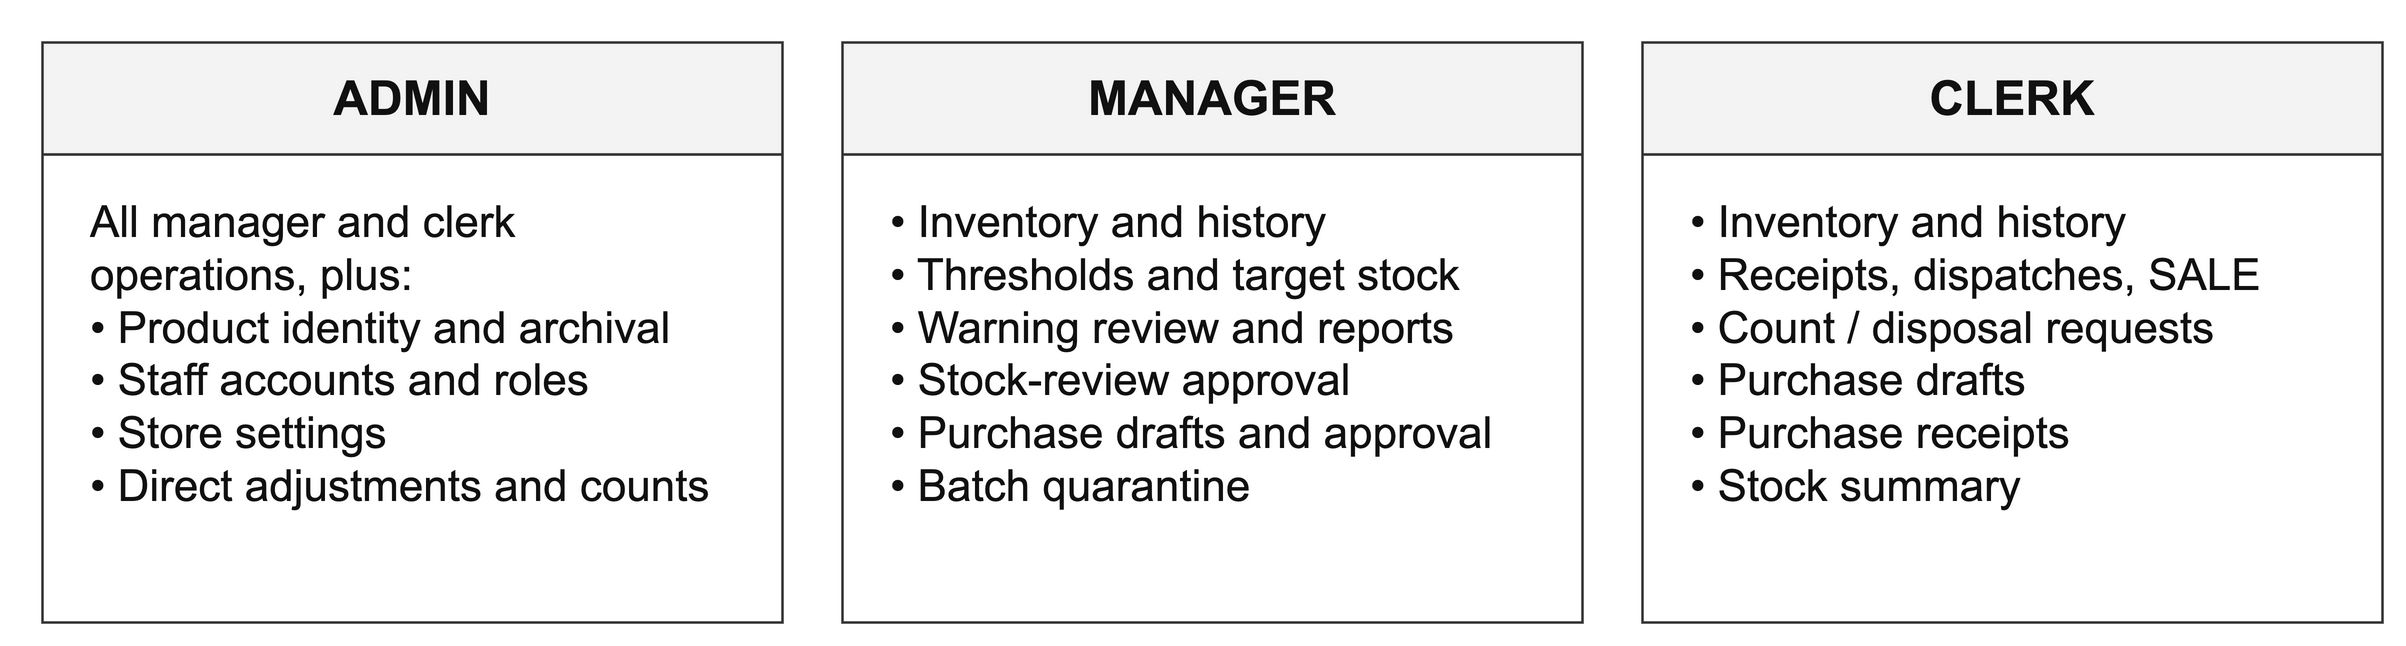
\includegraphics[width=\textwidth,height=0.70\textheight,keepaspectratio]{../figure-assets/diagrams/07-permission-model.png}
\caption{Fixed role bundles enforced by the server and reflected in navigation}\label{fig:permissions}
\end{figure}

\subsection{Catalog and inventory inspection}

Catalog administration requires unique SKUs, bounded non-negative prices, valid references and a consistent threshold hierarchy. Editing a product must not change its quantity, and archiving it must preserve its ledger while rejecting new movements. Category and supplier administration must protect existing references instead of silently detaching products on deletion.


Inventory inspection requires search by name, SKU and barcode, category selection, stock-health filters, stable sorting and bounded page sizes. The result count and pagination must describe the filtered selection, and an empty selection must offer a way to reset the filters.


For API consumers, pages are numbered from zero and their size is capped at one hundred; the interface loads twelve products per page. Sort fields are allow-listed and always end with an ID tie-breaker, which avoids ambiguous ordering and prevents a request parameter from becoming an arbitrary database expression. Snapshot consistency across pages is not promised while concurrent writes change the data.


\subsection{Stock operation requirements}

Each stock request must name a product, movement type, quantity, reason and idempotency key, while the actor is taken from the authenticated principal. The server must derive the signed effect and read the before balance under the product lock. A failed request must leave no accepted movement and no partial quantity change. An unchanged stocktake must still be recorded, because the observation itself carries information.


An exact replay must return the original transaction identifier without applying a second change, and reusing a key with different normalized content must produce a conflict. Requests that would make the quantity negative or exceed the supported maximum must be rejected. Concurrent dispatches must be serialized per product so that the successful ones can never oversell the locked balance.


\subsection{Warning and reporting requirements}

A sellable balance of zero must be classified as OUT, even when the threshold is also zero, and a positive balance equal to the reorder threshold must be LOW. Batch expiry reduces sellable quantity at the configured business-day boundary while the physical quantity remains available for disposal. A healthy replenishment must resolve the shortage and open a recovery episode. Slow-moving detection considers sales only, over a configured window. Continued low stock at the same severity must keep its reviewer, and any change to the threshold or warning policy must re-evaluate the affected episodes.


Reports must describe the recorded stock state rather than invent business indicators: inventory value uses current prices, the activity trend counts movements by UTC date, and the category mix uses current quantity totals. Acknowledgement must record who reviewed an episode without changing stock, and this distinction must be visible in labels, API operations and database relationships alike.


\FloatBarrier

\section{Non-functional requirements and quality boundaries}

Correctness takes priority over optional acceleration. MySQL must retain products, movements, warnings and settings, and neither posting stock nor retrieving authoritative warning results may depend on Redis. The movement path must update the balance, audit record, warning state and cache revision in one transaction, so that a failure rolls back the whole change instead of exposing a partial result.


The application must be reproducible from explicit dependencies and migrations. Local services are versioned in the repository, and evaluation scripts record machine, workload and sample metadata where available. Because another host may yield different latencies, reproducibility here means that the workload and procedure can be inspected and repeated, not that every recorded number will recur exactly.


Responsiveness is checked in a phone-sized viewport, with table scrolling confined to its container. The interface pairs stock colors with text labels and gives form fields descriptive names. These choices address relevant accessibility concerns, but full WCAG conformance is not claimed, since that would require a broader manual and automated assessment \citep{wcag}. Table~\ref{tab:quality} lists each quality attribute with the limits of its current evidence.


\begin{table}[htbp]\centering\small\setstretch{1.05}\setlength{\tabcolsep}{3pt}\renewcommand{\arraystretch}{1.25}
\caption{Quality requirements and limits of the current evidence}\label{tab:quality}
\begin{tabular}{>{\raggedright\arraybackslash}p{0.3\textwidth}>{\raggedright\arraybackslash}p{0.3\textwidth}>{\raggedright\arraybackslash}p{0.3\textwidth}}
\toprule
\textbf{Attribute} & \textbf{Required behavior} & \textbf{Current verification boundary} \\
\midrule
\leavevmode{}Consistency & \leavevmode{}Atomic bounded stock changes & \leavevmode{}Selected real-database transaction and concurrency cases \\
\leavevmode{}Retry handling & \leavevmode{}One accepted result per actor key and intention & \leavevmode{}Exact and conflicting replay plus same-product concurrency \\
\leavevmode{}Authorization & \leavevmode{}Server permission for each protected operation & \leavevmode{}Integration checks and browser guard scenarios \\
\leavevmode{}Recoverability & \leavevmode{}MySQL state remains authoritative without cache & \leavevmode{}Recorded Redis interruption and application restart \\
\leavevmode{}Usability & \leavevmode{}Clear stock semantics and recoverable empty states & \leavevmode{}Interface inspection and responsive browser checks \\
\leavevmode{}Performance & \leavevmode{}Described latency under a documented workload & \leavevmode{}Small sequential local warning-query benchmark \\
\leavevmode{}Maintainability & \leavevmode{}Explicit layers, schema and reproducible dependencies & \leavevmode{}Source structure, migrations and runnable scripts \\
\bottomrule\end{tabular}\end{table}

\FloatBarrier

\section{Analysis of related inventory systems}

\subsection{Reordering rules in Odoo}

Odoo's replenishment workflow uses minimum and maximum stock quantities to decide when, and how much, to reorder \citep{odoo}. Shelfwise similarly derives a replenishment suggestion from an explicit stock boundary, but the suggestion only seeds a draft purchase: submission, approval and receipt remain separate audited actions. Approval rechecks the current suggestion, and partial receipts create batch-aware movements. Supplier settlement and lead-time optimization are outside the implemented workflow.


\subsection{Retained ledger explanations in ERPNext}

ERPNext follows an immutable-ledger approach in which cancelling a document preserves the original entries and records reversing ones instead of deleting the earlier posting \citep{erpnext}. The underlying principle—accepted operational history must remain explainable after a correction—also guides Shelfwise, and ERPNext's stock ledger shows how such postings can be inspected within a larger enterprise system \citep{erpnext-stock}.


Shelfwise likewise keeps accepted movement rows and records corrections as later adjustments or stocktakes. Its audit history is, however, enforced only through the application's endpoints; a privileged database administrator can still alter stored rows directly. Document cancellation, backdated reposting and accounting integration, which ERPNext also provides, are outside Shelfwise's scope.


\subsection{Spreadsheet and broader enterprise alternatives}

A spreadsheet can serve a very small stock list well when a single person controls editing: it is easy to inspect and requires almost no deployment. The difficulty addressed here arises once several staff roles need coordinated writes, attributed changes and server-enforced permissions, which a shared worksheet could provide only with additional controls. This comparison is analytical rather than an experimental evaluation of a particular spreadsheet product.


Enterprise resource planning systems integrate inventory with purchasing, warehouse locations, finance and sales. Shelfwise instead concentrates on one store's inventory transactions, warning rules and reviewed stock workflows. The narrower scope reduces integration effort and leaves checkout, accounting and multi-store operation to later development. Table~\ref{tab:alternatives} summarizes the comparison.


\begin{table}[htbp]\centering\small\setstretch{1.05}\setlength{\tabcolsep}{3pt}\renewcommand{\arraystretch}{1.25}
\caption{Comparison of inventory-management approaches within the project scope}\label{tab:alternatives}
\begin{tabular}{>{\raggedright\arraybackslash}p{0.3\textwidth}>{\raggedright\arraybackslash}p{0.3\textwidth}>{\raggedright\arraybackslash}p{0.3\textwidth}}
\toprule
\textbf{Approach} & \textbf{Useful characteristics} & \textbf{Gap relative to this assignment} \\
\midrule
\leavevmode{}Shared stock worksheet & \leavevmode{}Simple deployment and direct visibility & \leavevmode{}Requires added controls for concurrency, roles and attributed changes \\
\leavevmode{}Documented Odoo replenishment & \leavevmode{}Quantity policies connected to replenishment & \leavevmode{}Broader enterprise and supplier scope \\
\leavevmode{}Documented ERPNext ledger & \leavevmode{}Retained posting and correction explanations & \leavevmode{}Broader document, accounting and reposting mechanisms \\
\leavevmode{}Shelfwise bounded application & \leavevmode{}Batch-aware stock, warning rules, review and purchase approval with tests & \leavevmode{}No checkout integration, accounting, multi-store isolation or store-user study \\
\bottomrule\end{tabular}\end{table}

\FloatBarrier

\section{Technology selection and comparative analysis}

\subsection{Backend and persistence}

Java 21 and Spring Boot 3.5.16 provide typed request records, validation, servlet security, JPA repositories, transaction management and health endpoints, within the Java and build-tool versions documented by the framework \citep{springboot}. The inventory-specific validation and consistency rules are implemented in the service layer.


MySQL serves as the durable relational store. Its locking reads provide a primitive for coordinating updates to a product row, and its constraints protect identities and foreign keys \citep{mysql-locks}. PostgreSQL could support an equivalent design; the choice reflects the existing project baseline and tested environment rather than a comparative benchmark. Flyway migrations define the schema, and JPA validates the mapping at startup.


Redis caches warning-page responses and nothing else. It follows the cache-aside pattern, in which a miss triggers an authoritative query and a best-effort cache fill \citep{redis-cache}. To prevent stale pages after a write, the project adds a revision namespace stored in the database. This adds a read to every query and a shared update to every relevant write, so the cache must be evaluated with these costs included rather than assumed to be faster.


\subsection{Frontend and communication}

Vue 3 provides a component-based browser interface, and TypeScript describes the response shapes used by pages and the API client \citep{vue}. Vue Router handles navigation, Pinia holds the authenticated account, Axios performs HTTP requests, Element Plus supplies the controls and ECharts renders the summaries. Responsive styles adapt the same application to desktop and phone-sized screens.


Shelfwise exposes a resource-oriented JSON API with server-side session authentication. Since Fielding lists stateless interaction among the REST constraints \citep{fielding2000}, the session-based API departs from REST in that the server retains request context. A second application node would therefore require shared sessions or session affinity.


\subsection{Development and verification tooling}

Docker Compose packages both the local and the release deployment: MySQL and Redis run as infrastructure services, Spring Boot runs in a Java runtime image, and Nginx serves the Vue bundle. A GitHub Actions workflow publishes the frontend and backend images and mirrors the pinned infrastructure images to GHCR for delivery to Windows hosts. Maven and Vite build the application, and Testcontainers, Vitest and Playwright support backend, frontend and browser verification. Table~\ref{tab:stack} lists the pinned versions.


\begin{table}[htbp]\centering\small\setstretch{1.05}\setlength{\tabcolsep}{3pt}\renewcommand{\arraystretch}{1.25}
\caption{Implemented technology baseline and responsibility}\label{tab:stack}
\begin{tabular}{>{\raggedright\arraybackslash}p{0.3\textwidth}>{\raggedright\arraybackslash}p{0.3\textwidth}>{\raggedright\arraybackslash}p{0.3\textwidth}}
\toprule
\textbf{Layer} & \textbf{Pinned technology} & \textbf{Responsibility} \\
\midrule
\leavevmode{}Backend & \leavevmode{}Java 21 and Spring Boot 3.5.16 & \leavevmode{}HTTP validation, security and transaction coordination \\
\leavevmode{}Persistence & \leavevmode{}Spring Data JPA and Flyway & \leavevmode{}Entity mapping, repository access and schema lifecycle \\
\leavevmode{}Database & \leavevmode{}MySQL 8.4.8 & \leavevmode{}Durable records, constraints and locking \\
\leavevmode{}Cache & \leavevmode{}Redis 7.4.9 & \leavevmode{}Optional thirty-second warning-page cache \\
\leavevmode{}Browser & \leavevmode{}Vue 3.5.22 and TypeScript 5.9.3 & \leavevmode{}Reactive interface and typed client data \\
\leavevmode{}UI and charts & \leavevmode{}Element Plus 2.11.5 and ECharts 6.1.0 & \leavevmode{}Controls and stock visualizations \\
\leavevmode{}Frontend build & \leavevmode{}Vite 7.3.6 and project Node 22 baseline & \leavevmode{}Development proxy and asset build \\
\leavevmode{}Evaluation & \leavevmode{}JUnit, Testcontainers, Vitest and Playwright & \leavevmode{}Layer-specific executable checks \\
\bottomrule\end{tabular}\end{table}

\FloatBarrier

\section{Chapter summary}

The requirements define an auditable stock intention, a warning review independent of stock, and a single durable source of truth. Odoo and ERPNext illustrate replenishment policy and retained ledger history, and the technology analysis shows how the narrower scope of this project can be implemented. Chapter 3 translates the requirements into an architecture and relational constraints that make each acceptance condition observable.

\chapter{DESIGN}
\section{System architecture design}
The system is a modular monolith with a Vue browser client, Spring Boot application, MySQL database, and Redis cache. The browser submits intentions; the server validates role, reason, quantity, and idempotency; MySQL commits durable state; Redis may serve a versioned warning page. This layout makes the source of truth explicit and avoids distributing a single stock balance across services.
\fig[0.48]{architecture.png}{Runtime architecture and data ownership.}{fig:aligned-architecture}
\section{Refining the architecture design}
The backend is divided into authentication, catalog, inventory transaction, warning, and reporting responsibilities. The request path locks one product before calculating a new balance. A successful movement changes quantity, writes the ledger, evaluates warning state, and increments the cache revision in one transaction. A cache read uses the revision, warning type, lifecycle state, page, and size as its key. Redis failures fall back to MySQL.
\fig[0.54]{stock-workflow.png}{Stock movement transaction and warning update flow.}{fig:aligned-workflow}
\section{Database design}
Products reference categories and optional suppliers. Inventory transactions reference products and actors. Warning episodes reference products and optional reviewers. Unique constraints protect SKU, barcode, username, and actor/idempotency-key combinations. Product quantity is bounded at the database and service layers. Historical products are archived instead of deleted.
\section{Role permission model}
\begin{table}[H]\centering\small\caption{Role permission model.}\begin{tabularx}{\textwidth}{Yccc}\toprule Operation & Administrator & Manager & Clerk\\\midrule Read inventory/history & Yes & Yes & Yes\\ Post stock movement & Yes & No & Yes\\ Edit product identity & Yes & No & No\\ Edit thresholds & Yes & Yes & No\\ Review warnings/reports & Yes & Yes & No\\ Manage users/settings & Yes & No & No\\\bottomrule\end{tabularx}\end{table}
\section{Security layered architecture}
Authentication uses a server session, BCrypt password hashes, CSRF tokens for unsafe browser methods, and server-side role checks. A request filter reloads the current enabled user and role from MySQL, so access changes apply without trusting an old session authority. The security model follows the basic role-bundle idea of RBAC~\citep{sandhu1996}. It does not claim production-grade MFA, rate limiting, password recovery, or penetration testing.

\chapter{IMPLEMENTATION}
\section{Development of information system classes}
The backend contains domain entities, repositories, validated request records, response records, controllers, a central inventory service, and security configuration. Flyway creates the schema and JPA validates it at startup. The service owns the stock transaction boundary. Quantity is not writable through catalog input. The startup demonstration seed runs only for an empty user table and requires an explicit local password.
\section{Development of software routing and paths}
The API includes authentication, dashboard, products, categories, suppliers, transactions, warnings, users, settings, and report paths. Product queries support search, category, health, archive, page, size, and allow-listed sort parameters. Transaction requests use a movement type, quantity, reason, and idempotency key. Warning requests accept lifecycle/type filters and a cache bypass parameter for evaluation.
\section{Implementation of software functions}
The dashboard reports current product count, low-stock count, out-of-stock count, estimated current-price value, movement count, recent activity, category mix, and priority warnings. The inventory view supports empty states, filters, pagination, CSV export, and product administration. The stock form distinguishes positive receiving/dispatch quantities, signed adjustments, and absolute counts. The warning board shows quantity, threshold, detection time, reviewer, and acknowledgement state.
\fig[0.45]{ui-dashboard.png}{Implemented dashboard for the current store state.}{fig:aligned-dashboard}
\fig[0.45]{ui-warnings.png}{Implemented warning board with independent review status.}{fig:aligned-warnings}
\section{Version control and semantic versioning management}
The project uses logical commits for bootstrap, design, inventory implementation, frontend implementation, thesis evidence, and layout corrections. The public repository excludes SPEC.md, local environment files, databases, dependencies, and build intermediates. Release tags identify the submission package and the later portrait-page and compact-pagination corrections.
\section{Information system deploying}
Docker Compose starts MySQL and Redis. The backend runs with Java 21 and Maven, while the frontend runs with Node 22 and Vite during development. A clean setup copies .env.example, starts containers, runs migration at application startup, and launches the browser client. Production deployment would require TLS, secure cookies, a secrets manager, backups, rate limiting, and a shared session strategy for multiple application nodes.

\chapter{System testing and evaluation}

\FloatBarrier

\section{Evaluation questions and evidence organization}

Evaluation addresses the four questions introduced at the beginning of the thesis. Functional tests examine whether stock changes are bounded and attributed. Concurrency and replay tests examine whether repeated or competing intentions produce acceptable results. Warning tests examine the separation of severity, recovery and review. Browser checks examine presentation and navigation. Local measurements and recorded failure scenarios examine the optional cache path and durable state.


The evidence has several dates and purposes. The backend and frontend result images included here are from 5 October 2026. The original browser acceptance record and performance and recovery records are dated 3 October UTC, corresponding to the local development session that produced them. A later capture run on 5 October obtains the expanded interface collection without posting new business data. These records are not interchangeable samples of one experiment.


\begingroup\small\setstretch{1.05}\setlength{\tabcolsep}{3pt}\renewcommand{\arraystretch}{1.25}
\begin{longtable}{>{\raggedright\arraybackslash}p{0.3\textwidth}>{\raggedright\arraybackslash}p{0.3\textwidth}>{\raggedright\arraybackslash}p{0.3\textwidth}}
\caption{Evaluation evidence and its scope}\label{tab:evidence-dates}\\
\toprule
\textbf{Evidence} & \textbf{Recorded date} & \textbf{What it establishes} \\
\midrule\endfirsthead
\toprule
\textbf{Evidence} & \textbf{Recorded date} & \textbf{What it establishes} \\
\midrule\endhead
\bottomrule\endfoot
Backend result log & 5 October 2026 local time & Twenty-seven integration cases completed without failures \\
Frontend result log & 5 October 2026 local time & Three threshold presentation tests passed \\
Original browser journey & 3 October 2026 UTC & Fourteen checks including one receipt and one acknowledgement \\
Expanded figure capture & 5 October 2026 UTC & Twenty-seven captures role guard checks and no page runtime errors \\
Warning-query benchmark & 3 October 2026 UTC & Six hundred sequential measured samples per mode \\
Redis interruption & 3 October 2026 UTC & Equivalent warning result during the recorded cache outage \\
Restart fingerprint & Preserved repository record & Equal selected product and transaction rows after restart \\
\end{longtable}\endgroup

The prototype uses fictitious records and local services. Tests can provide strong evidence for a specified invariant while still leaving practical questions unanswered. In particular, the study does not measure store-user learning, business losses avoided, supplier lead times or production capacity. The result discussion keeps the units and scope of each claim aligned with the recorded procedure.


\FloatBarrier

\section{Backend integration testing}

\FloatBarrier

\subsection{Environment and case coverage}

The backend test class uses Testcontainers to create MySQL and Redis instances for the test execution. Its dynamic properties direct the Spring application to those instances. This is valuable because locking, uniqueness and persistence behavior involve the actual database rather than an in-memory substitute. It does not mean that every production database setting or fault mode is reproduced.


The current integration suite contains 46 cases covering authentication, CSRF, role restrictions, catalogue validation, quantity changes, audit history, retry behavior, concurrency, shortage transitions, batch allocation, expiry policy, slow-moving detection, purchase approval, partial receipts, stock reviews and account safeguards. The result in Figure~\ref{fig:backend-result} reports zero failures, errors and skipped tests for the recorded run. A passing suite means that those executable assertions held in this run. It is not a numerical code-coverage percentage or a proof that all possible requests are correct.


\begin{figure}[htbp]\centering
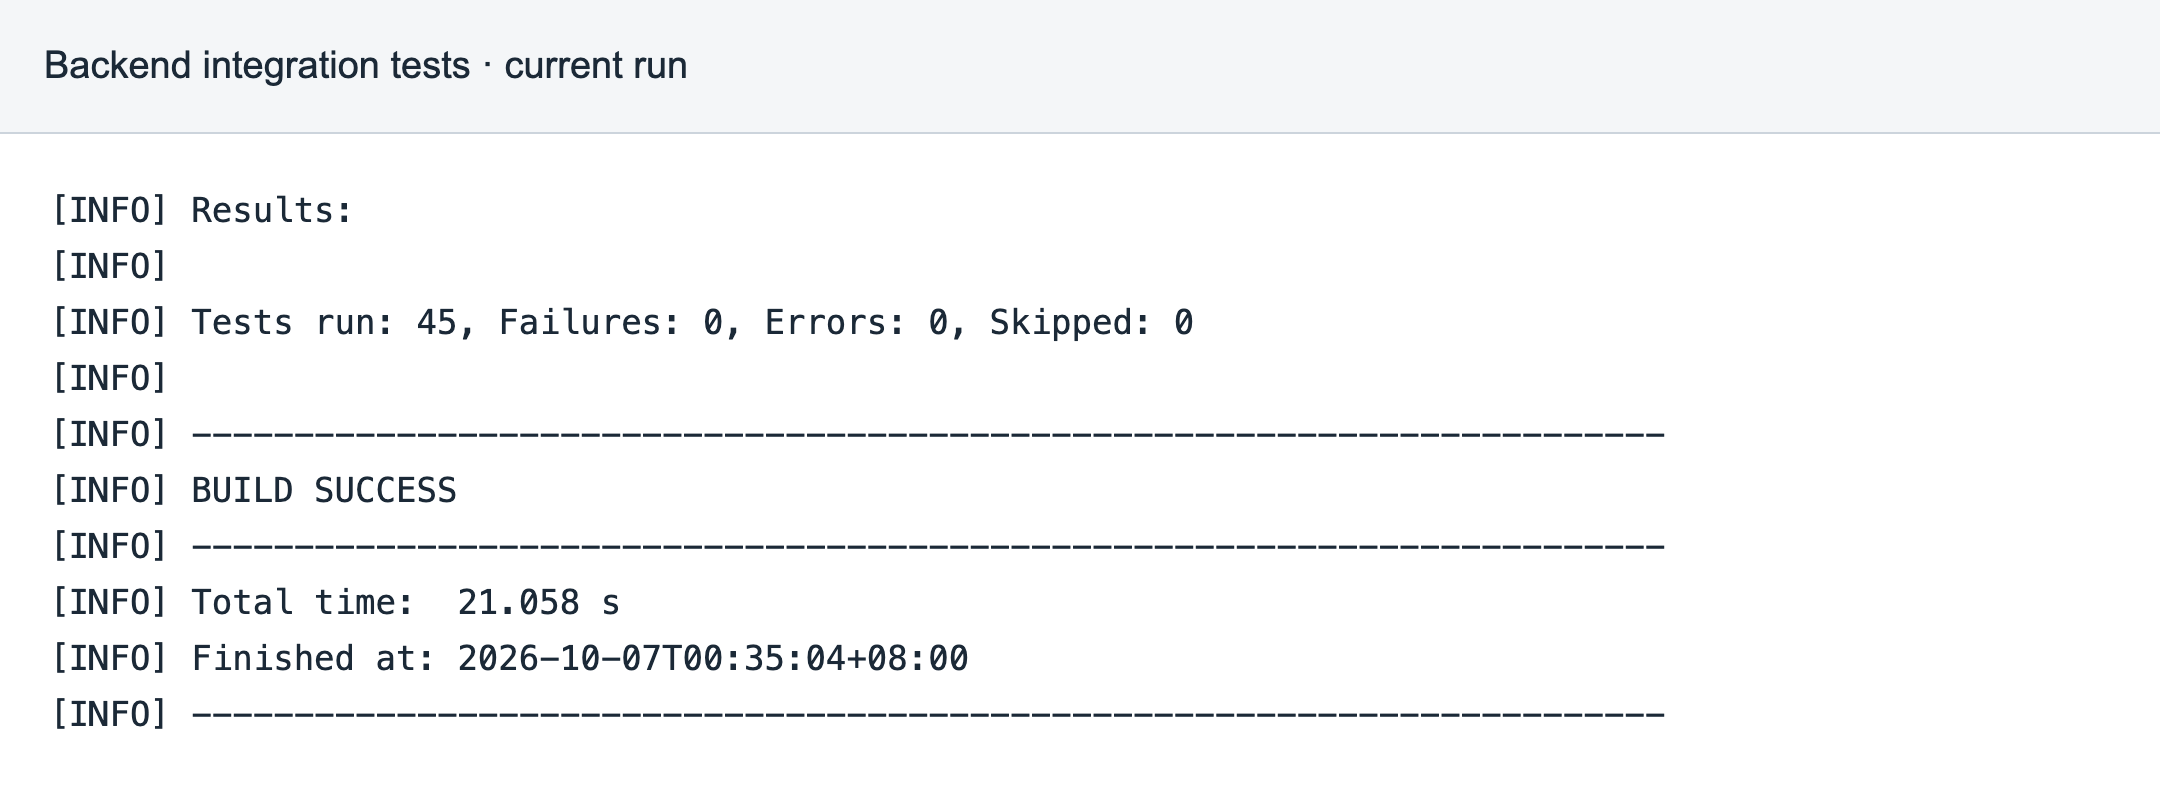
\includegraphics[width=\textwidth,height=0.40\textheight,keepaspectratio]{../figure-assets/evidence/01-backend-tests.png}
\caption{Backend integration result from the 5 October 2026 execution}\label{fig:backend-result}
\end{figure}

\begingroup\small\setstretch{1.05}\setlength{\tabcolsep}{3pt}\renewcommand{\arraystretch}{1.25}
\begin{longtable}{>{\raggedright\arraybackslash}p{0.3\textwidth}>{\raggedright\arraybackslash}p{0.3\textwidth}>{\raggedright\arraybackslash}p{0.3\textwidth}}
\caption{Main backend acceptance groups}\label{tab:backend-groups}\\
\toprule
\textbf{Group} & \textbf{Representative assertions} & \textbf{Reported outcome} \\
\midrule\endfirsthead
\toprule
\textbf{Group} & \textbf{Representative assertions} & \textbf{Reported outcome} \\
\midrule\endhead
\bottomrule\endfoot
Authentication & Anonymous denial invalid credentials and missing login fields & Passed \\
Authorization & Clerk review denial manager posting denial and threshold boundary & Passed \\
Catalogue & Unique SKU valid threshold hierarchy and archived movement denial & Passed \\
Stock arithmetic & Receipt dispatch signed adjustment absolute count and zero count & Passed \\
Audit behavior & Before and after history and unchanged stocktake observation & Passed \\
Retries & Equal replay identifier and changed-payload conflict & Passed \\
Concurrency & No overselling identical submission and first reviewer preservation & Passed \\
Warnings & Zero equality healthy recovery severity renewal and accurate filters & Passed \\
Administration & Last enabled administrator cannot be disabled or demoted & Passed \\
\end{longtable}\endgroup

\FloatBarrier

\subsection{Negative-stock and audit consistency}

The insufficient-stock test attempts a dispatch from an empty product. It expects a domain exception, unchanged transaction count and unchanged quantity. This checks both the arithmetic boundary and the absence of an accepted history row for a rejected operation. The receipt-and-dispatch test then verifies a valid sequence: before zero, receipt eight, dispatch three and final quantity five with two movements.


The absolute-count cases verify the semantic distinction from a relative adjustment. Starting at ten, an adjustment of negative two produces eight; counting three then produces delta negative five and after quantity three. Counting to zero is also accepted and auditable. An unchanged count creates a zero-delta history row. These cases would not be equivalent to a generic test that an input number can be stored in a product field.


\FloatBarrier

\subsection{Duplicate and concurrent requests}

The exact-replay case sends the same actor-scoped request twice and checks the same movement identifier and one stock effect. A changed quantity with that key produces a conflict. These assertions connect the returned response to the stored result rather than merely checking that the server returns a success status.


The concurrency source in Figure~\ref{fig:concurrency-code} shows two demanding scenarios. Twelve unit dispatch attempts compete for a starting balance of seven; the test expects exactly seven successes and quantity zero. Four concurrent identical stock-in submissions must produce one identifier and quantity four. Those bounds directly test the intended outcome under the selected same-product workload.


\begin{figure}[htbp]\centering
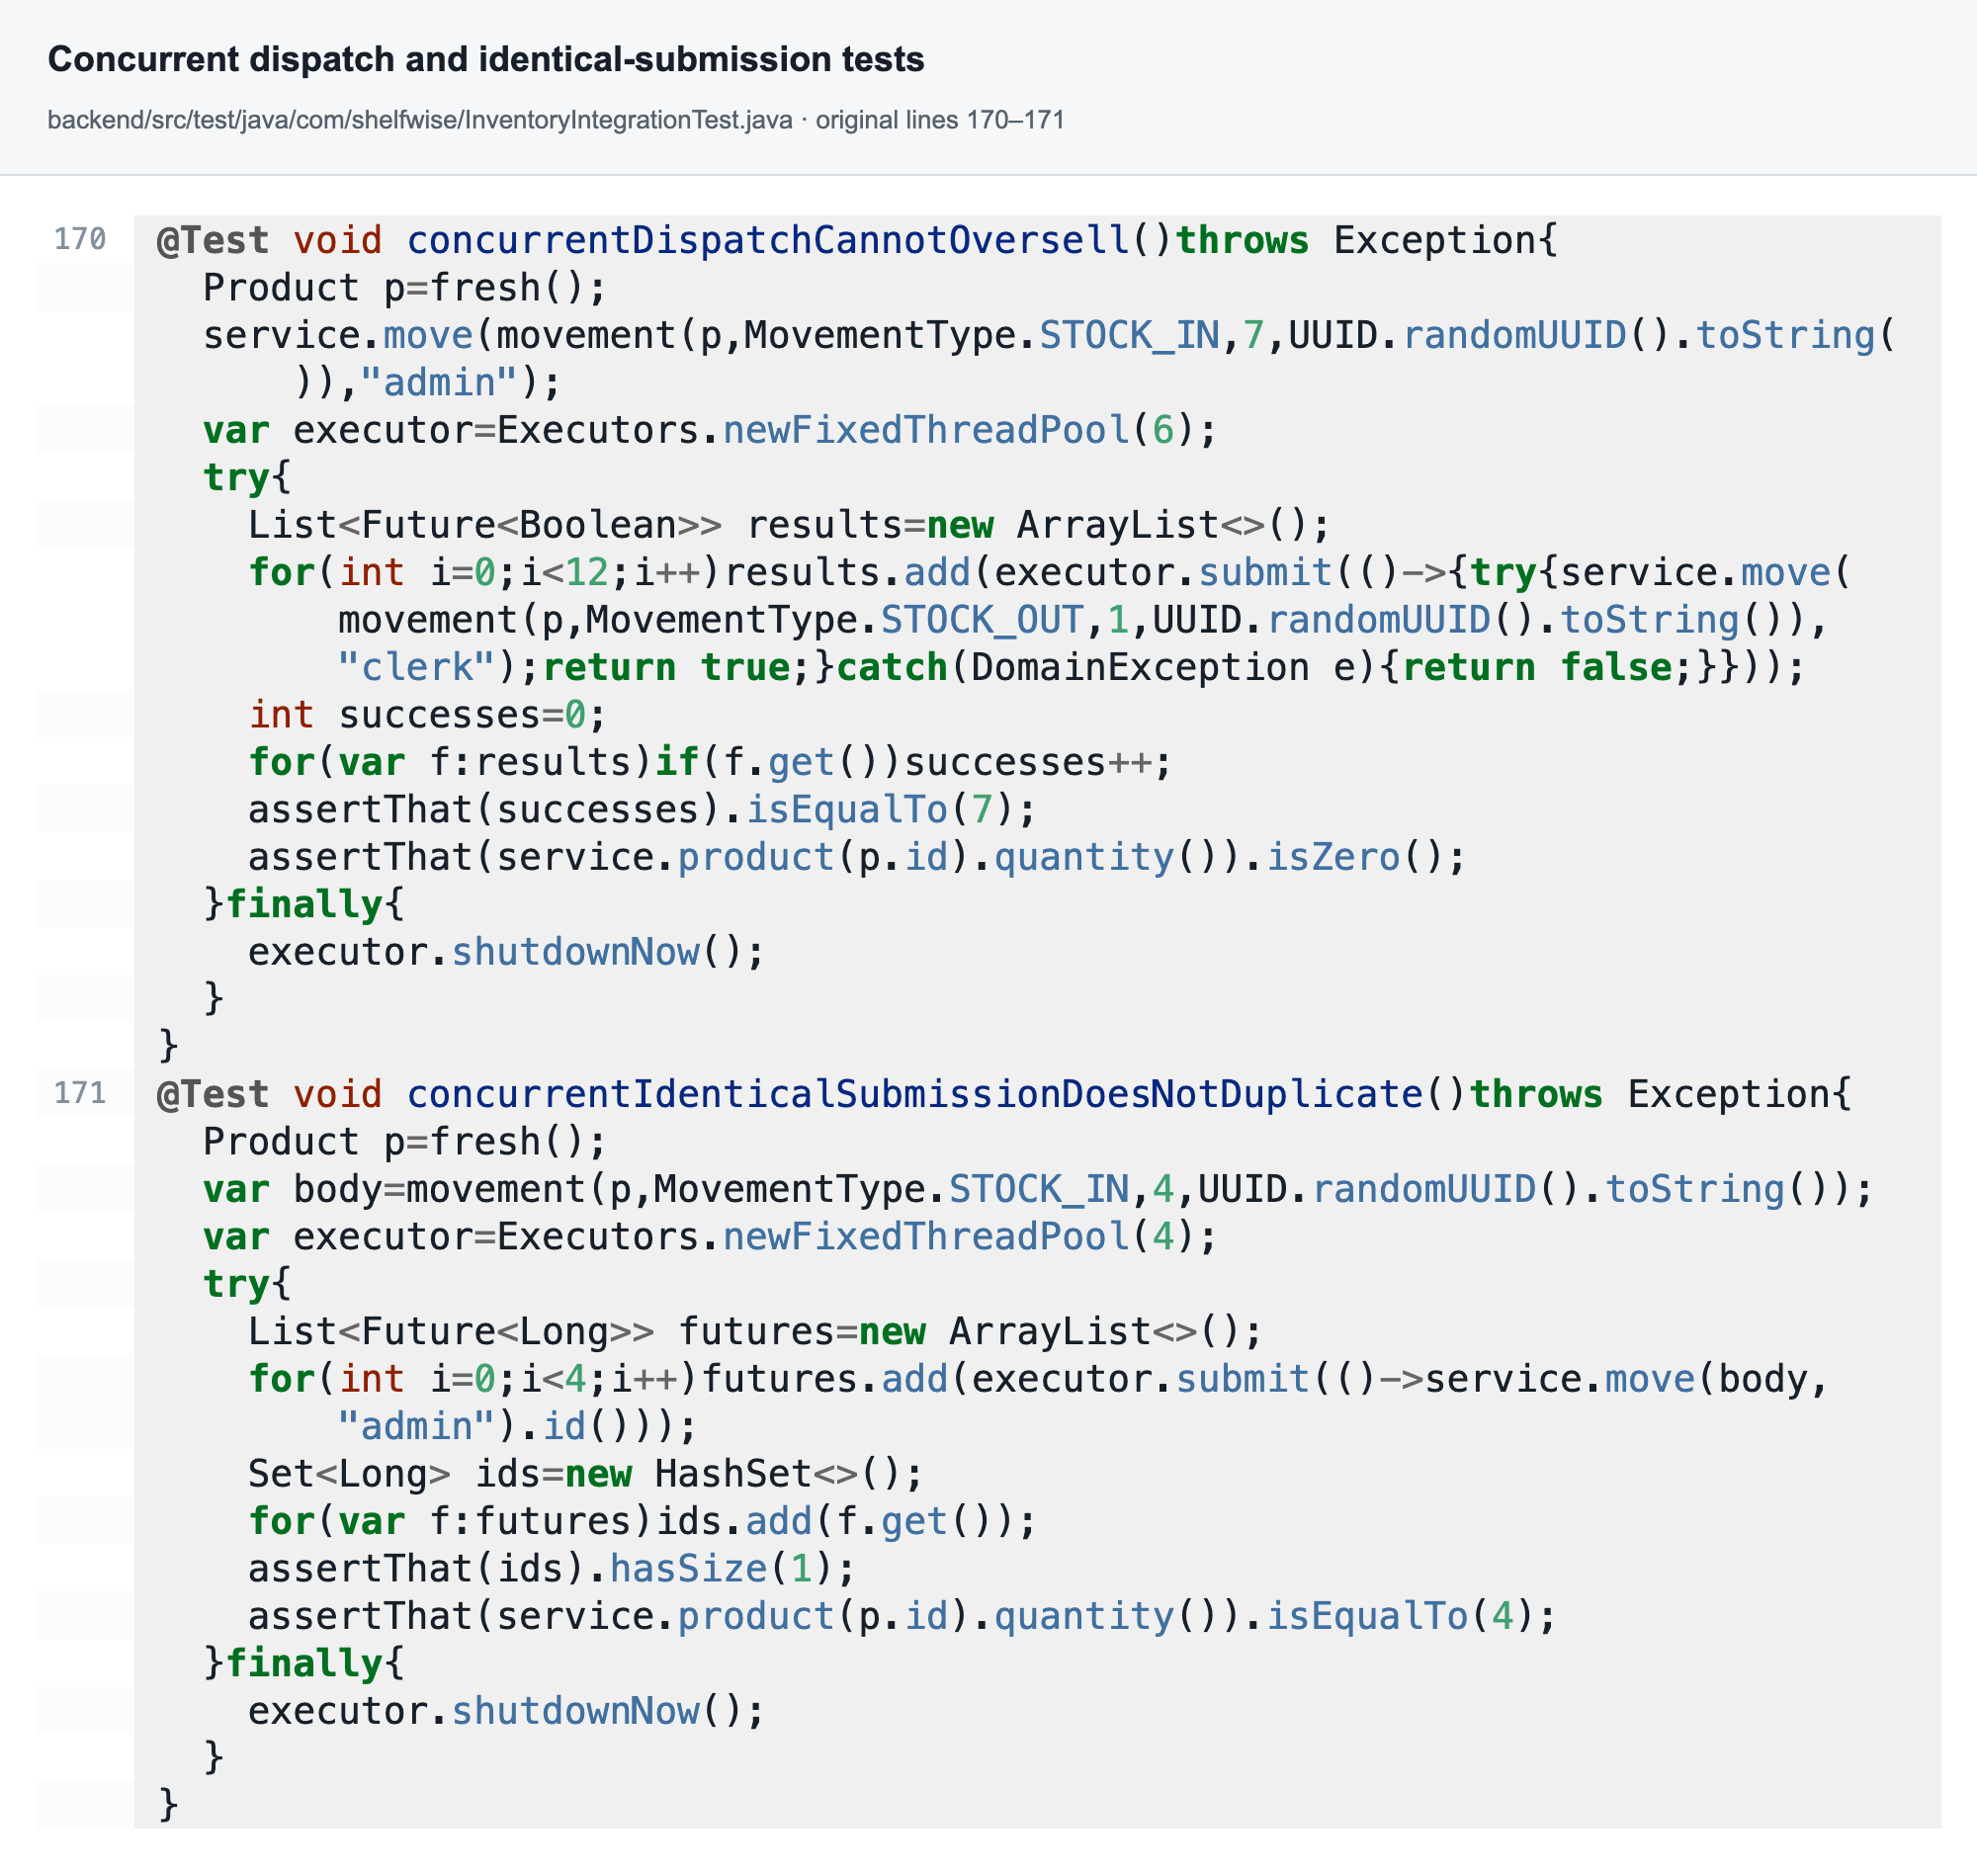
\includegraphics[width=\textwidth,height=0.84\textheight,keepaspectratio]{../figure-assets/code/12-code-concurrency-tests.png}
\caption{Actual concurrent dispatch and identical-submission integration cases}\label{fig:concurrency-code}
\end{figure}

The tests do not establish fairness, sustained throughput or behavior under every lock timeout. The shared revision row can serialize parts of writes across different products. Cross-product reuse of one actor-key pair and database deadlocks require additional targeted cases. MySQL's documentation treats deadlocks as a transaction condition that applications must consider \citep{mysql-deadlocks}; the current service does not advertise an automatic deadlock-retry policy.


\FloatBarrier

\subsection{Warning and review assertions}

The threshold test verifies OUT at zero and LOW at exact positive equality. Healthy replenishment removes the active shortage and creates RESTOCKED. Expiry tests verify the inclusive expiry-day boundary under the configured timezone, and slow-moving tests verify that sales-only history forms one continuous event. A review test verifies that acknowledgement becomes visible through the cache and leaves quantity zero. The concurrent-review case expects both responses to expose the same first reviewer. Archive cases confirm that the product rejects movements and its open warnings are resolved.


The recovery test named for restocked expiry and new shortage exercises renewed shortage after replenishment. Separate expiry tests exercise business-day boundaries, invalid timezone rejection and expiry-aware sellable balances. They do not establish a long-running scheduler reliability distribution. The supported conclusion is that the implemented rules agree at the tested boundaries; broader clock, cache and operational scheduling workloads remain future work.


\FloatBarrier

\section{Batch, purchasing and review workflow testing}

The expanded backend cases exercise receipt metadata replay, concurrent receipts, FEFO/FIFO batch allocation, exclusion of expired or quarantined batches, and disposal approval after a batch remainder changes. These assertions connect physical stock to sellable stock rather than checking only a product-level integer.


Purchase tests cover multi-line draft creation, rejection and edit, completion, partial receipt, receipt replay, cancellation and concurrent approval. Approval rechecks the current replenishment suggestion before accepting a quantity. A receipt is therefore both a purchasing event and an audited stock movement; replay must not create a second batch or movement.


Stock-review tests cover count and disposal submissions, stale snapshots, idempotent submissions, long bounded reasons and role denials. The approval path applies a movement only after the stored snapshot or batch remainder is still valid. These cases are stronger evidence for the expanded workflow than a screenshot of a review button, but they remain synthetic single-store scenarios.


\FloatBarrier

\section{Frontend and browser testing}

\FloatBarrier

\subsection{Threshold presentation}

The frontend unit tests check the zero boundary, exact threshold equality and positive healthy stock. The source in Figure~\ref{fig:frontend-test-code} makes those values visible. The result in Figure~\ref{fig:frontend-result} confirms three passing cases. The tests protect the labels shown beside quantity so that the browser does not contradict the server's fundamental classification.


\begin{figure}[htbp]\centering
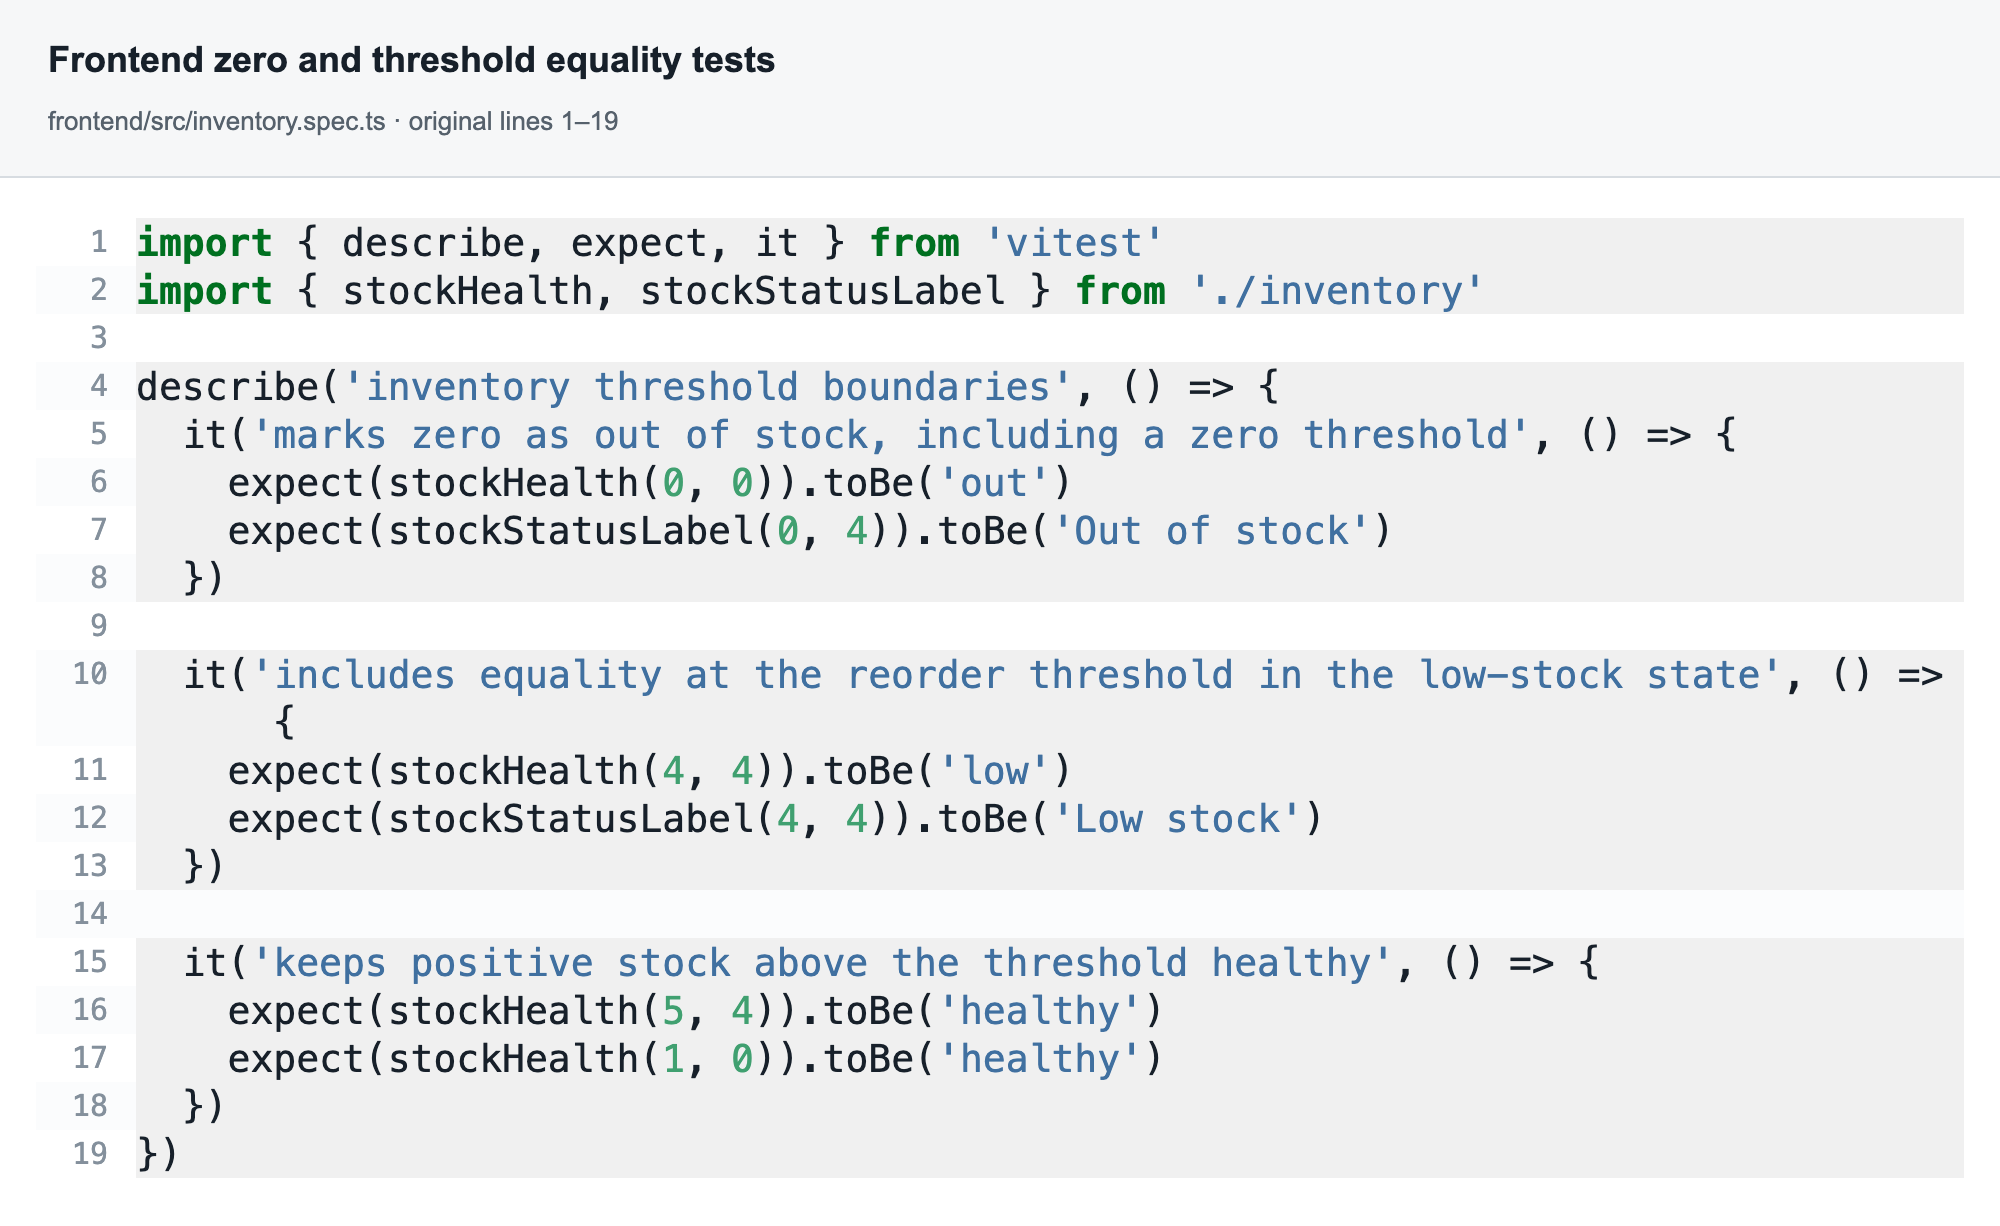
\includegraphics[width=\textwidth,height=0.84\textheight,keepaspectratio]{../figure-assets/code/13-code-boundary-tests.png}
\caption{Frontend test inputs for zero equality and healthy stock}\label{fig:frontend-test-code}
\end{figure}

\begin{figure}[htbp]\centering
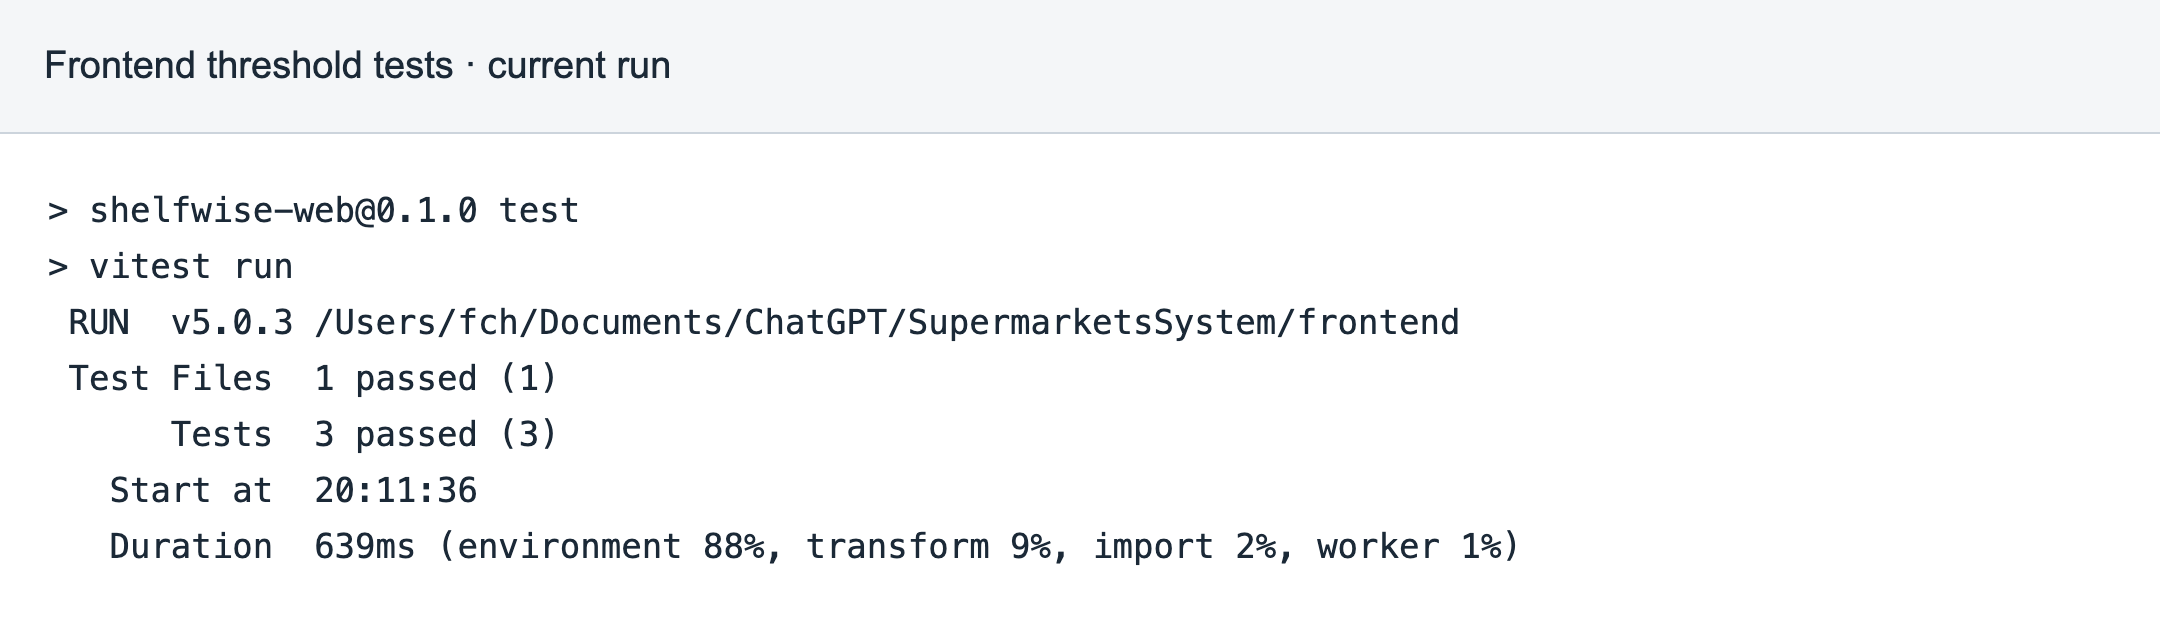
\includegraphics[width=\textwidth,height=0.40\textheight,keepaspectratio]{../figure-assets/evidence/02-frontend-tests.png}
\caption{Frontend unit-test result from the current execution}\label{fig:frontend-result}
\end{figure}

These are small focused tests. They do not cover every modal, asynchronous loading state or component interaction. The broader browser journeys serve a complementary purpose by opening the application and observing rendered behavior. Neither layer establishes full accessibility conformance or practical usability for store employees.


\FloatBarrier

\subsection{Earlier operational browser journey}

The preserved earlier browser record contains fourteen checks with zero JavaScript runtime errors. It covers administrator login and operational views, an empty search, an actual receipt submission with the correct delta, clerk and manager navigation restrictions, managerial acknowledgement and phone-sized viewport containment. Its write operations make it stronger evidence of an interface-to-server journey than a collection of screenshots alone.


The empty-result interface in Figure~\ref{fig:empty-ui} illustrates the recovery state used by the search check. It presents an explanation and a way to clear filters. A successful empty selection should not be confused with a failed request; error handling and query results represent different conditions in the application.


\begin{figure}[htbp]\centering
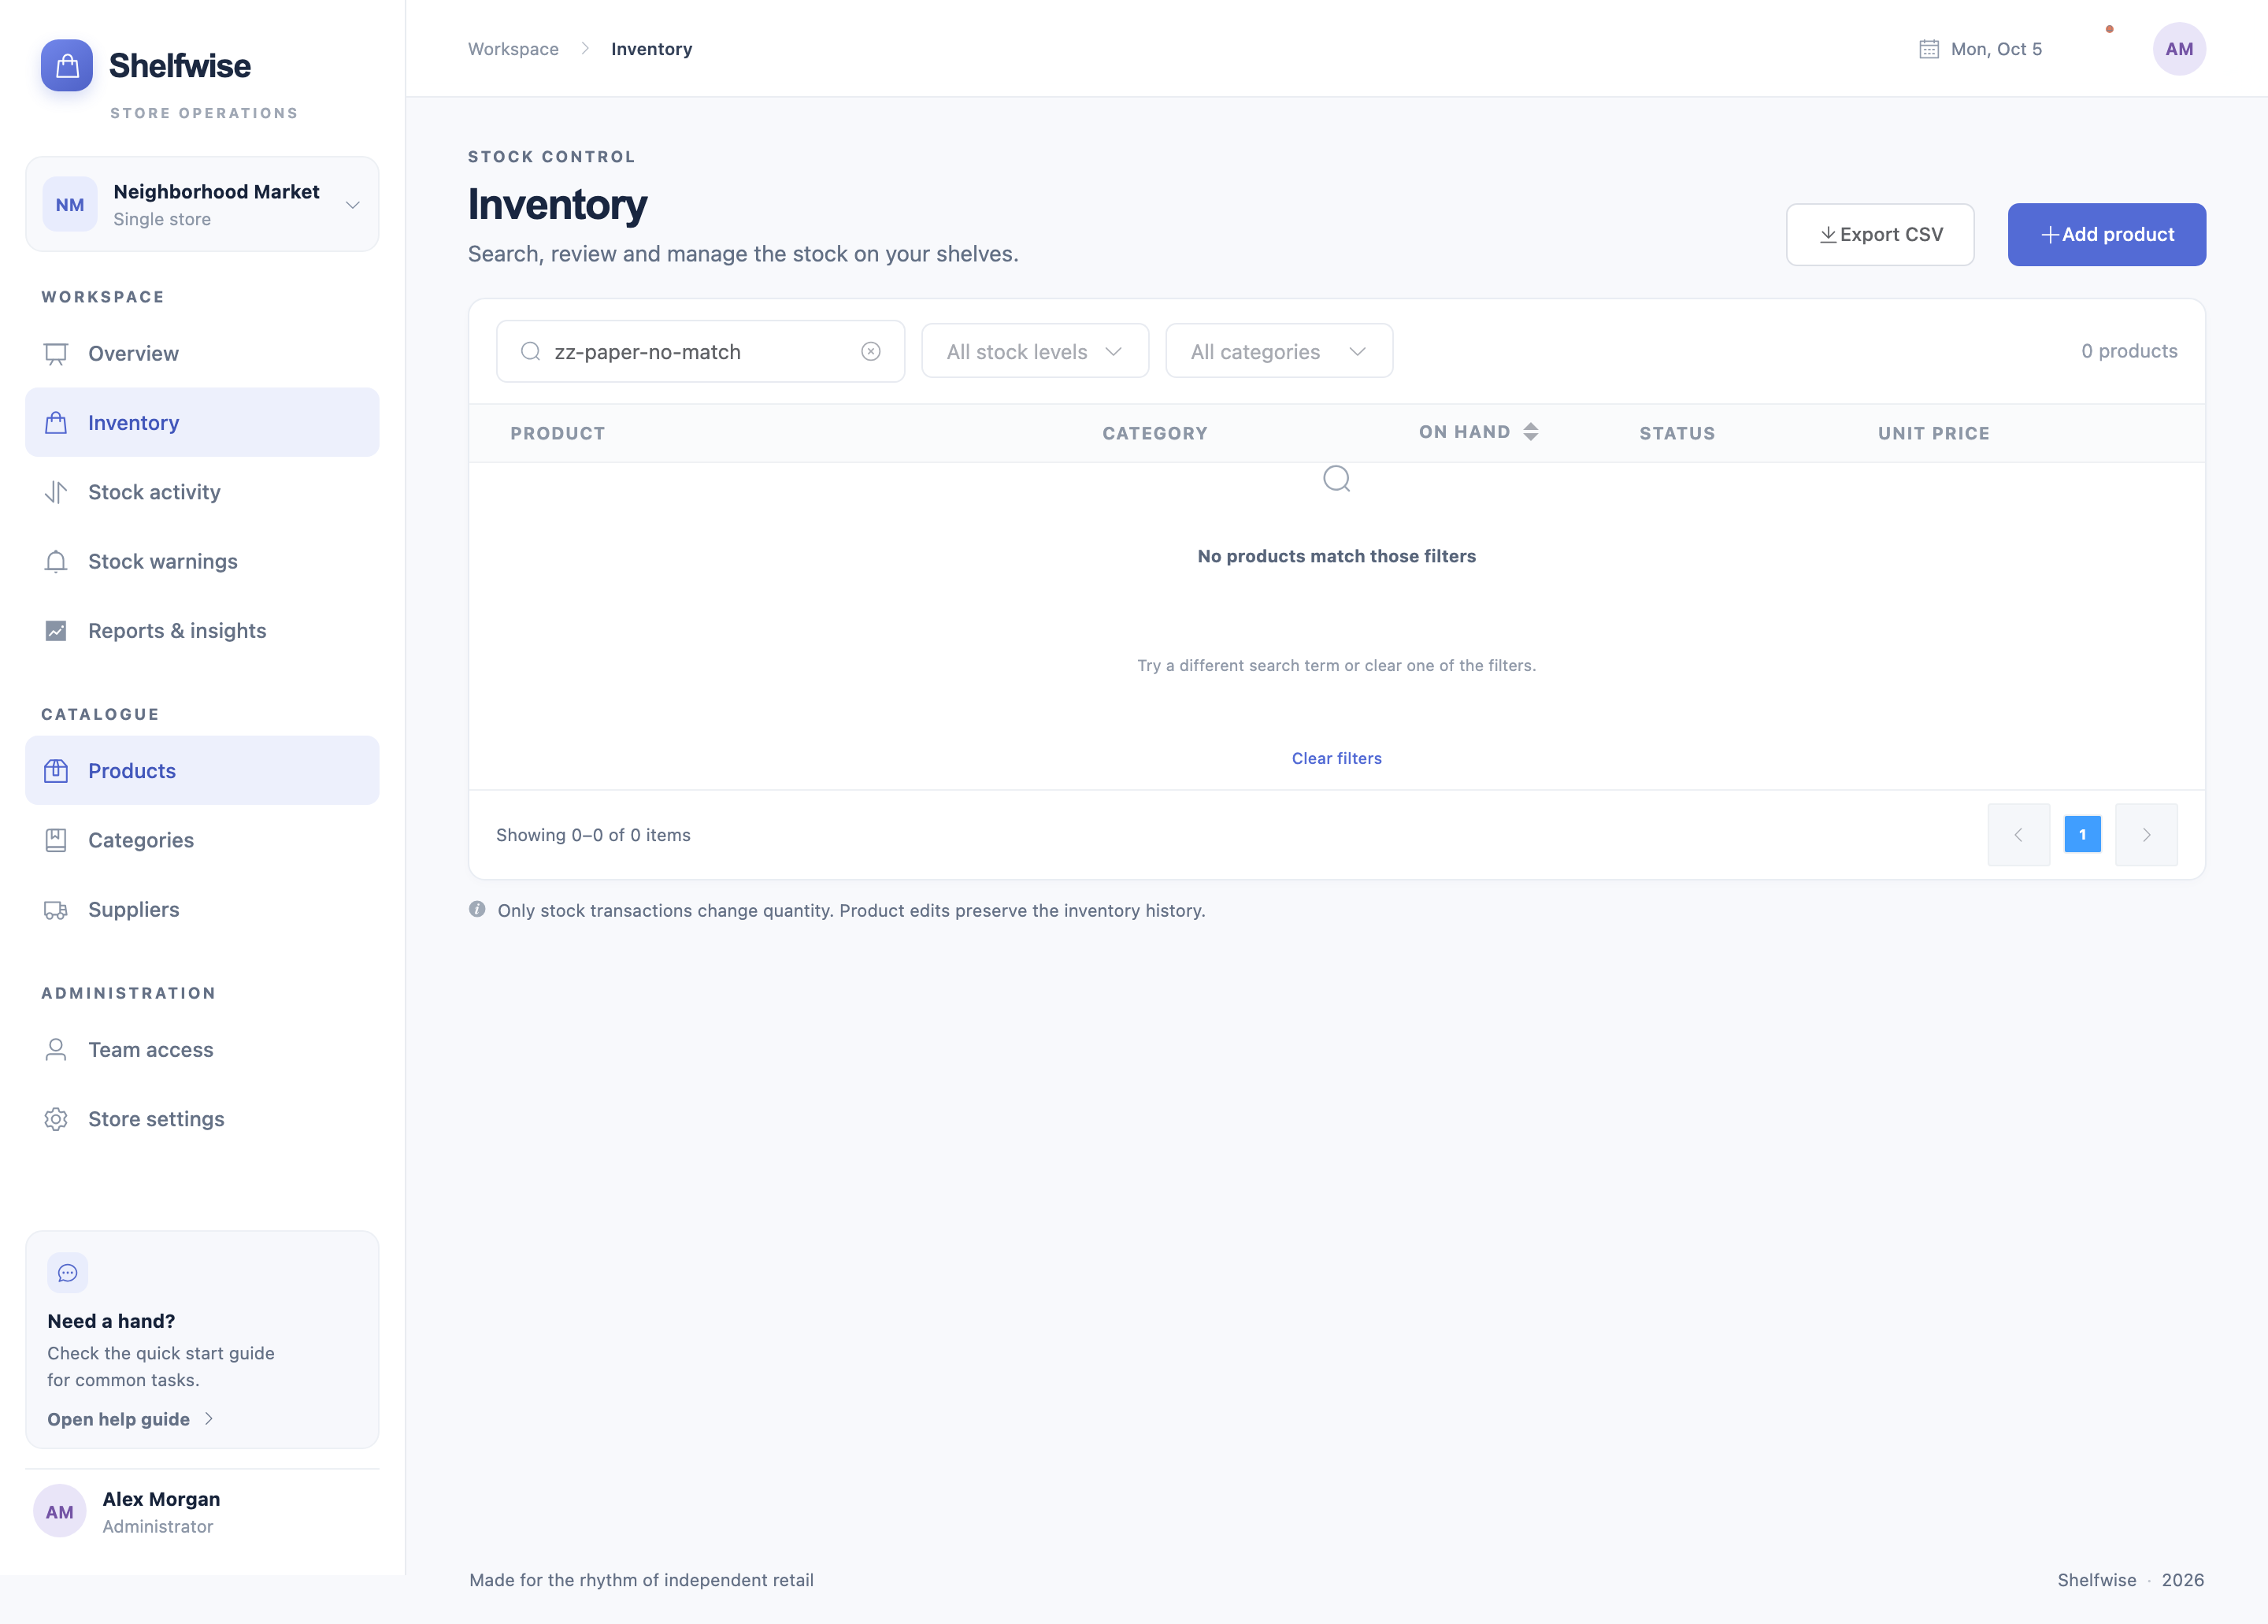
\includegraphics[width=\textwidth,height=0.40\textheight,keepaspectratio]{../figure-assets/ui/13-empty-search.png}
\caption{Empty inventory search with a visible recovery action}\label{fig:empty-ui}
\end{figure}

\FloatBarrier

\subsection{Expanded capture verification}

The later capture run obtains twenty-seven interfaces and forms. It signs in as all three roles, checks that managers cannot reach staff administration and clerks cannot reach the warning board, and checks document width at 390 pixels. It records zero page runtime errors. The verification image in Figure~\ref{fig:browser-result} identifies this capture-specific evidence.


\begin{figure}[htbp]\centering
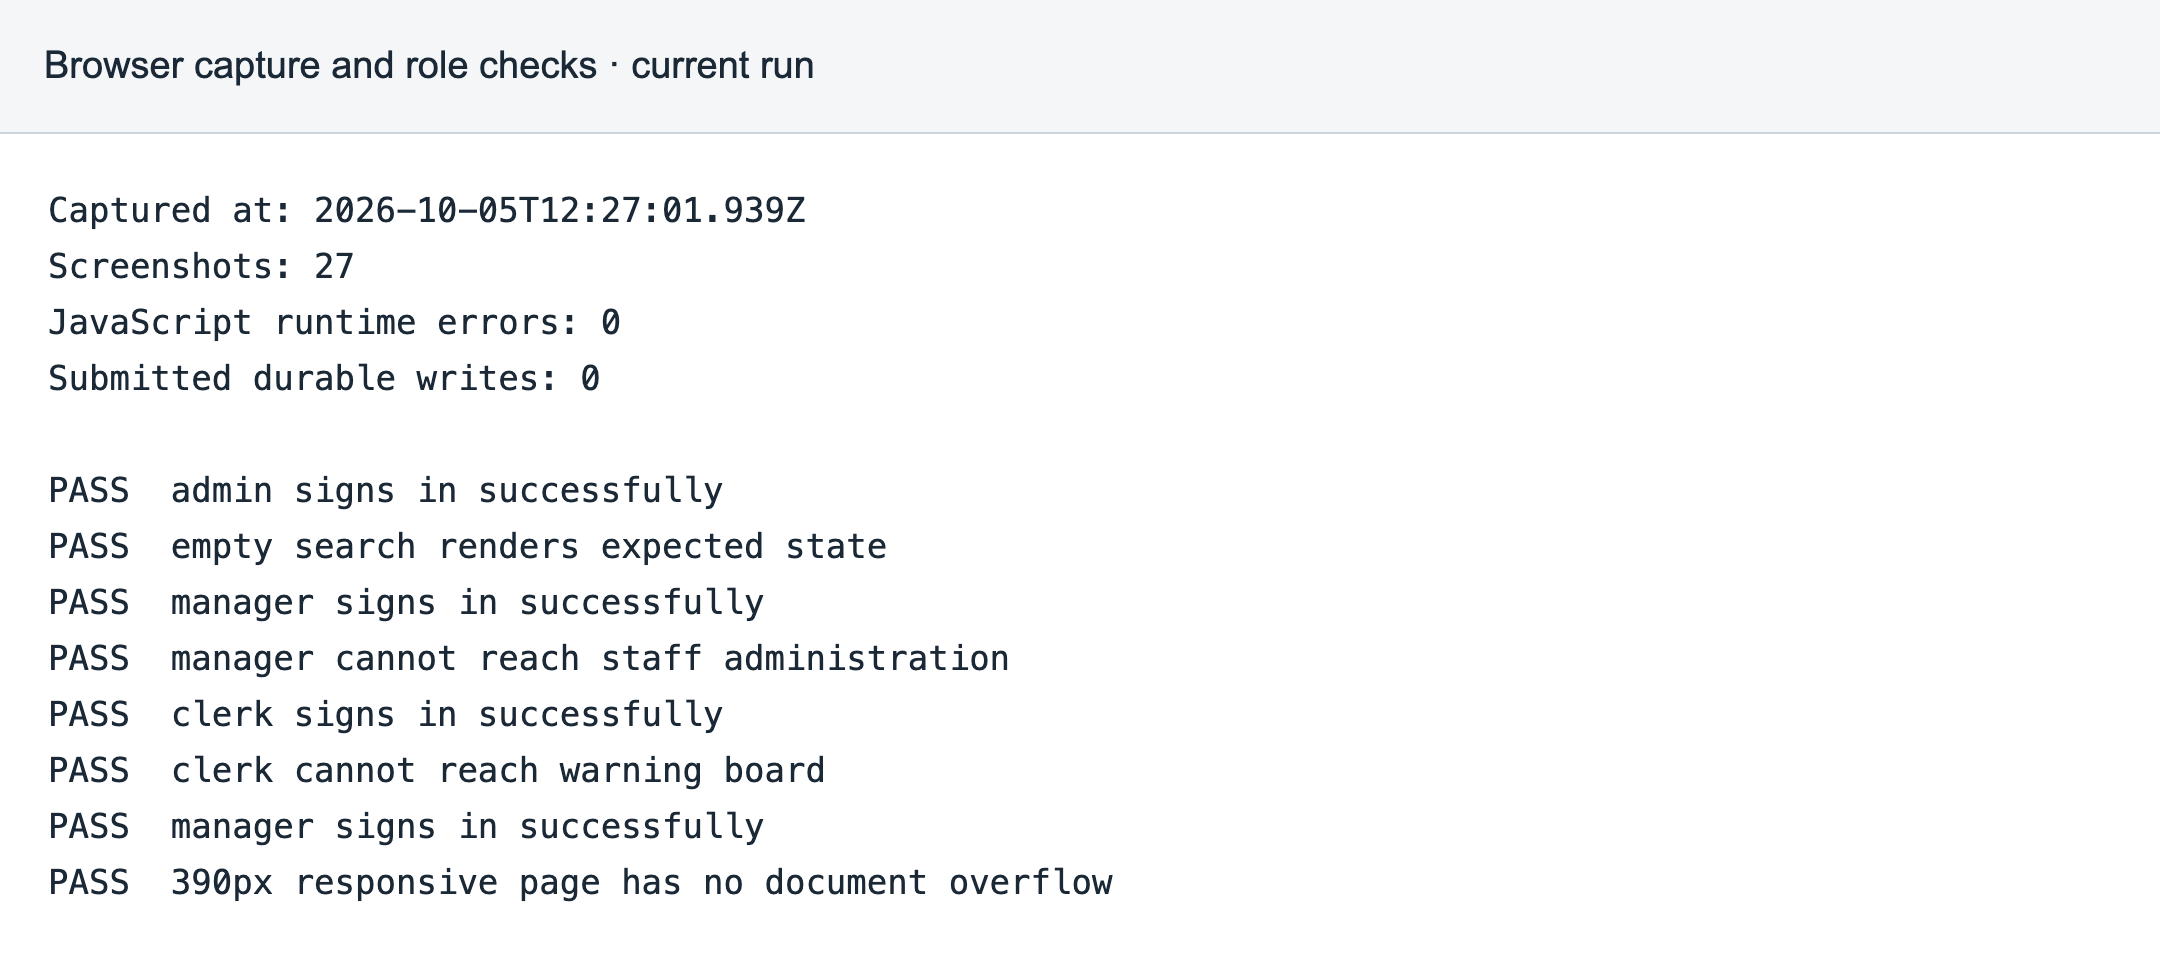
\includegraphics[width=\textwidth,height=0.40\textheight,keepaspectratio]{../figure-assets/evidence/03-browser-verification.png}
\caption{Capture-run checks and the absence of posted business changes}\label{fig:browser-result}
\end{figure}

The capture process opens forms and fills drafts but does not submit stock, account or catalogue changes. Receipt and dispatch images therefore demonstrate the implemented controls and labels, not additional accepted movements. The thesis uses the earlier operational journey and backend cases when discussing accepted writes. This separation allows screenshots to remain useful without assigning them evidential weight they do not have.


\FloatBarrier

\section{Performance test of the warning query}

\FloatBarrier

\subsection{Workload and measurement procedure}

The performance record compares the warning query with cache enabled and with cache bypassed. It uses sixteen products, sixteen open warning episodes, page size one hundred and concurrency one. Three rounds alternate the mode order. Each mode receives twenty warm-up requests and two hundred measured requests per round, giving six hundred measured samples for each mode. Results include the local HTTP path rather than isolated Redis or MySQL operation time.


The recorded host is Apple Silicon macOS with MySQL and Redis containers accessed over loopback. The script records the operating system, machine type, Python version and backend/database baseline. Authentication, durable revision retrieval, filtering, serialization and network handling can contribute to each response. A cache hit therefore avoids only part of the total request work.


\begingroup\small\setstretch{1.05}\setlength{\tabcolsep}{3pt}\renewcommand{\arraystretch}{1.25}
\begin{longtable}{>{\raggedright\arraybackslash}p{0.45\textwidth}>{\raggedright\arraybackslash}p{0.45\textwidth}}
\caption{Recorded local benchmark workload}\label{tab:benchmark-workload}\\
\toprule
\textbf{Parameter} & \textbf{Value} \\
\midrule\endfirsthead
\toprule
\textbf{Parameter} & \textbf{Value} \\
\midrule\endhead
\bottomrule\endfoot
Products & 16 \\
Open warning episodes & 16 \\
Page size & 100 \\
Concurrent requests & 1 \\
Alternating measurement rounds & 3 \\
Warm-up requests per mode per round & 20 \\
Measured requests per mode per round & 200 \\
Pooled measured samples per mode & 600 \\
Network and service placement & Loopback HTTP and local Colima containers \\
\end{longtable}\endgroup

The benchmark is preserved evidence, not a newly executed production experiment. The inclusion of warm-up and alternating order improves interpretability, but it does not remove all variation due to the host, containers or background activity. No simultaneous-user or capacity curve can be inferred from sequential requests.


\FloatBarrier

\subsection{Descriptive latency results}

The summary in Table~\ref{tab:latency} reports pooled median and tail percentiles from the preserved samples. Percentiles use the sorted-sample index implemented by the project's evaluation script. The Redis-enabled path has a median of approximately 5.33 ms, compared with approximately 6.56 ms for bypass. Its p95 is approximately 7.57 ms, compared with 8.11 ms. These are measurements in this particular run, not latency targets guaranteed by the architecture.


\begingroup\small\setstretch{1.05}\setlength{\tabcolsep}{3pt}\renewcommand{\arraystretch}{1.25}
\begin{longtable}{>{\raggedright\arraybackslash}p{0.18\textwidth}>{\raggedright\arraybackslash}p{0.18\textwidth}>{\raggedright\arraybackslash}p{0.18\textwidth}>{\raggedright\arraybackslash}p{0.18\textwidth}>{\raggedright\arraybackslash}p{0.18\textwidth}}
\caption{Warning-query latency from six hundred samples per mode}\label{tab:latency}\\
\toprule
\textbf{Mode} & \textbf{Samples} & \textbf{Median ms} & \textbf{p95 ms} & \textbf{p99 ms} \\
\midrule\endfirsthead
\toprule
\textbf{Mode} & \textbf{Samples} & \textbf{Median ms} & \textbf{p95 ms} & \textbf{p99 ms} \\
\midrule\endhead
\bottomrule\endfoot
Redis enabled & 600 & 5.33 & 7.57 & 8.87 \\
MySQL bypass & 600 & 6.56 & 8.11 & 9.42 \\
\end{longtable}\endgroup

The bar chart in Figure~\ref{fig:latency-summary} presents the same descriptive statistics. It helps separate the typical result from the upper-tail values. The approximately 1.24 ms difference between pooled medians is small in absolute terms. It is associated with the optional cache path under this dataset, while the benchmark includes costs that the cache cannot remove.


\begin{figure}[htbp]\centering
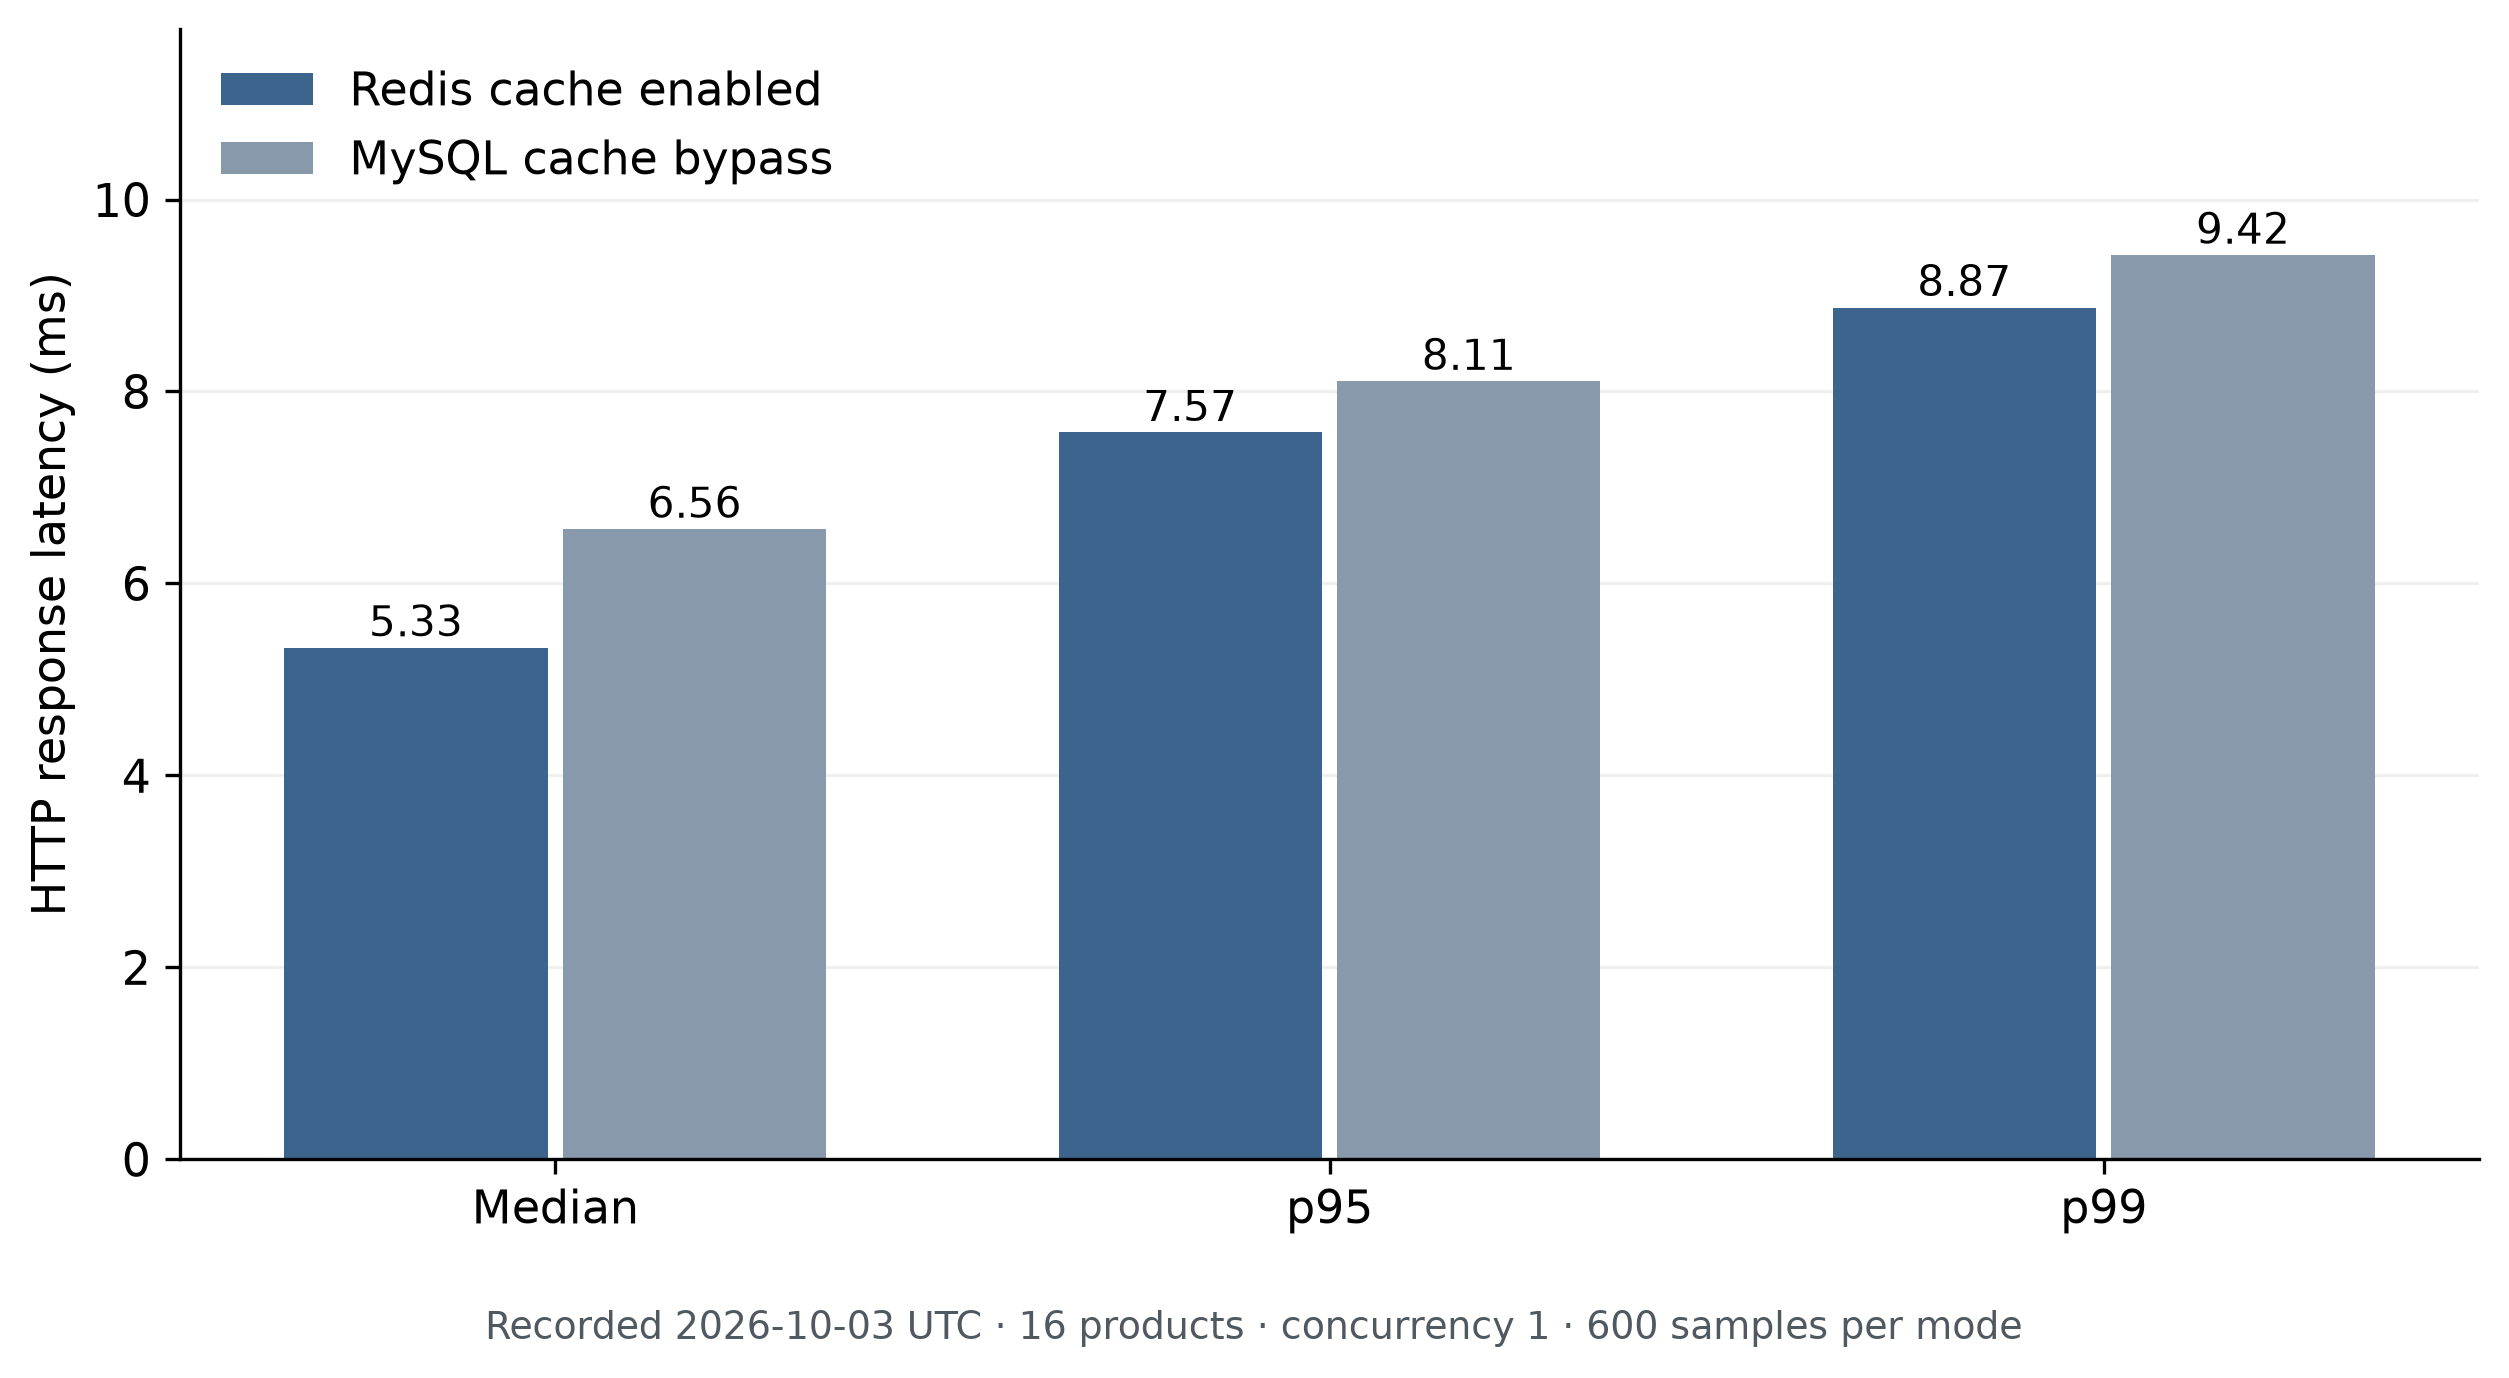
\includegraphics[width=\textwidth,height=0.40\textheight,keepaspectratio]{../figure-assets/evidence/04-latency-summary.png}
\caption{Pooled local median and tail latency for cached and bypass warning queries}\label{fig:latency-summary}
\end{figure}

The empirical cumulative distribution in Figure~\ref{fig:latency-ecdf} shows the proportion of measured responses below each latency. It reveals overlapping distributions instead of implying that every cached request is faster than every bypass request. The plotted tail also makes occasional slower observations visible. No statistical hypothesis test or confidence interval is reported.


\begin{figure}[htbp]\centering
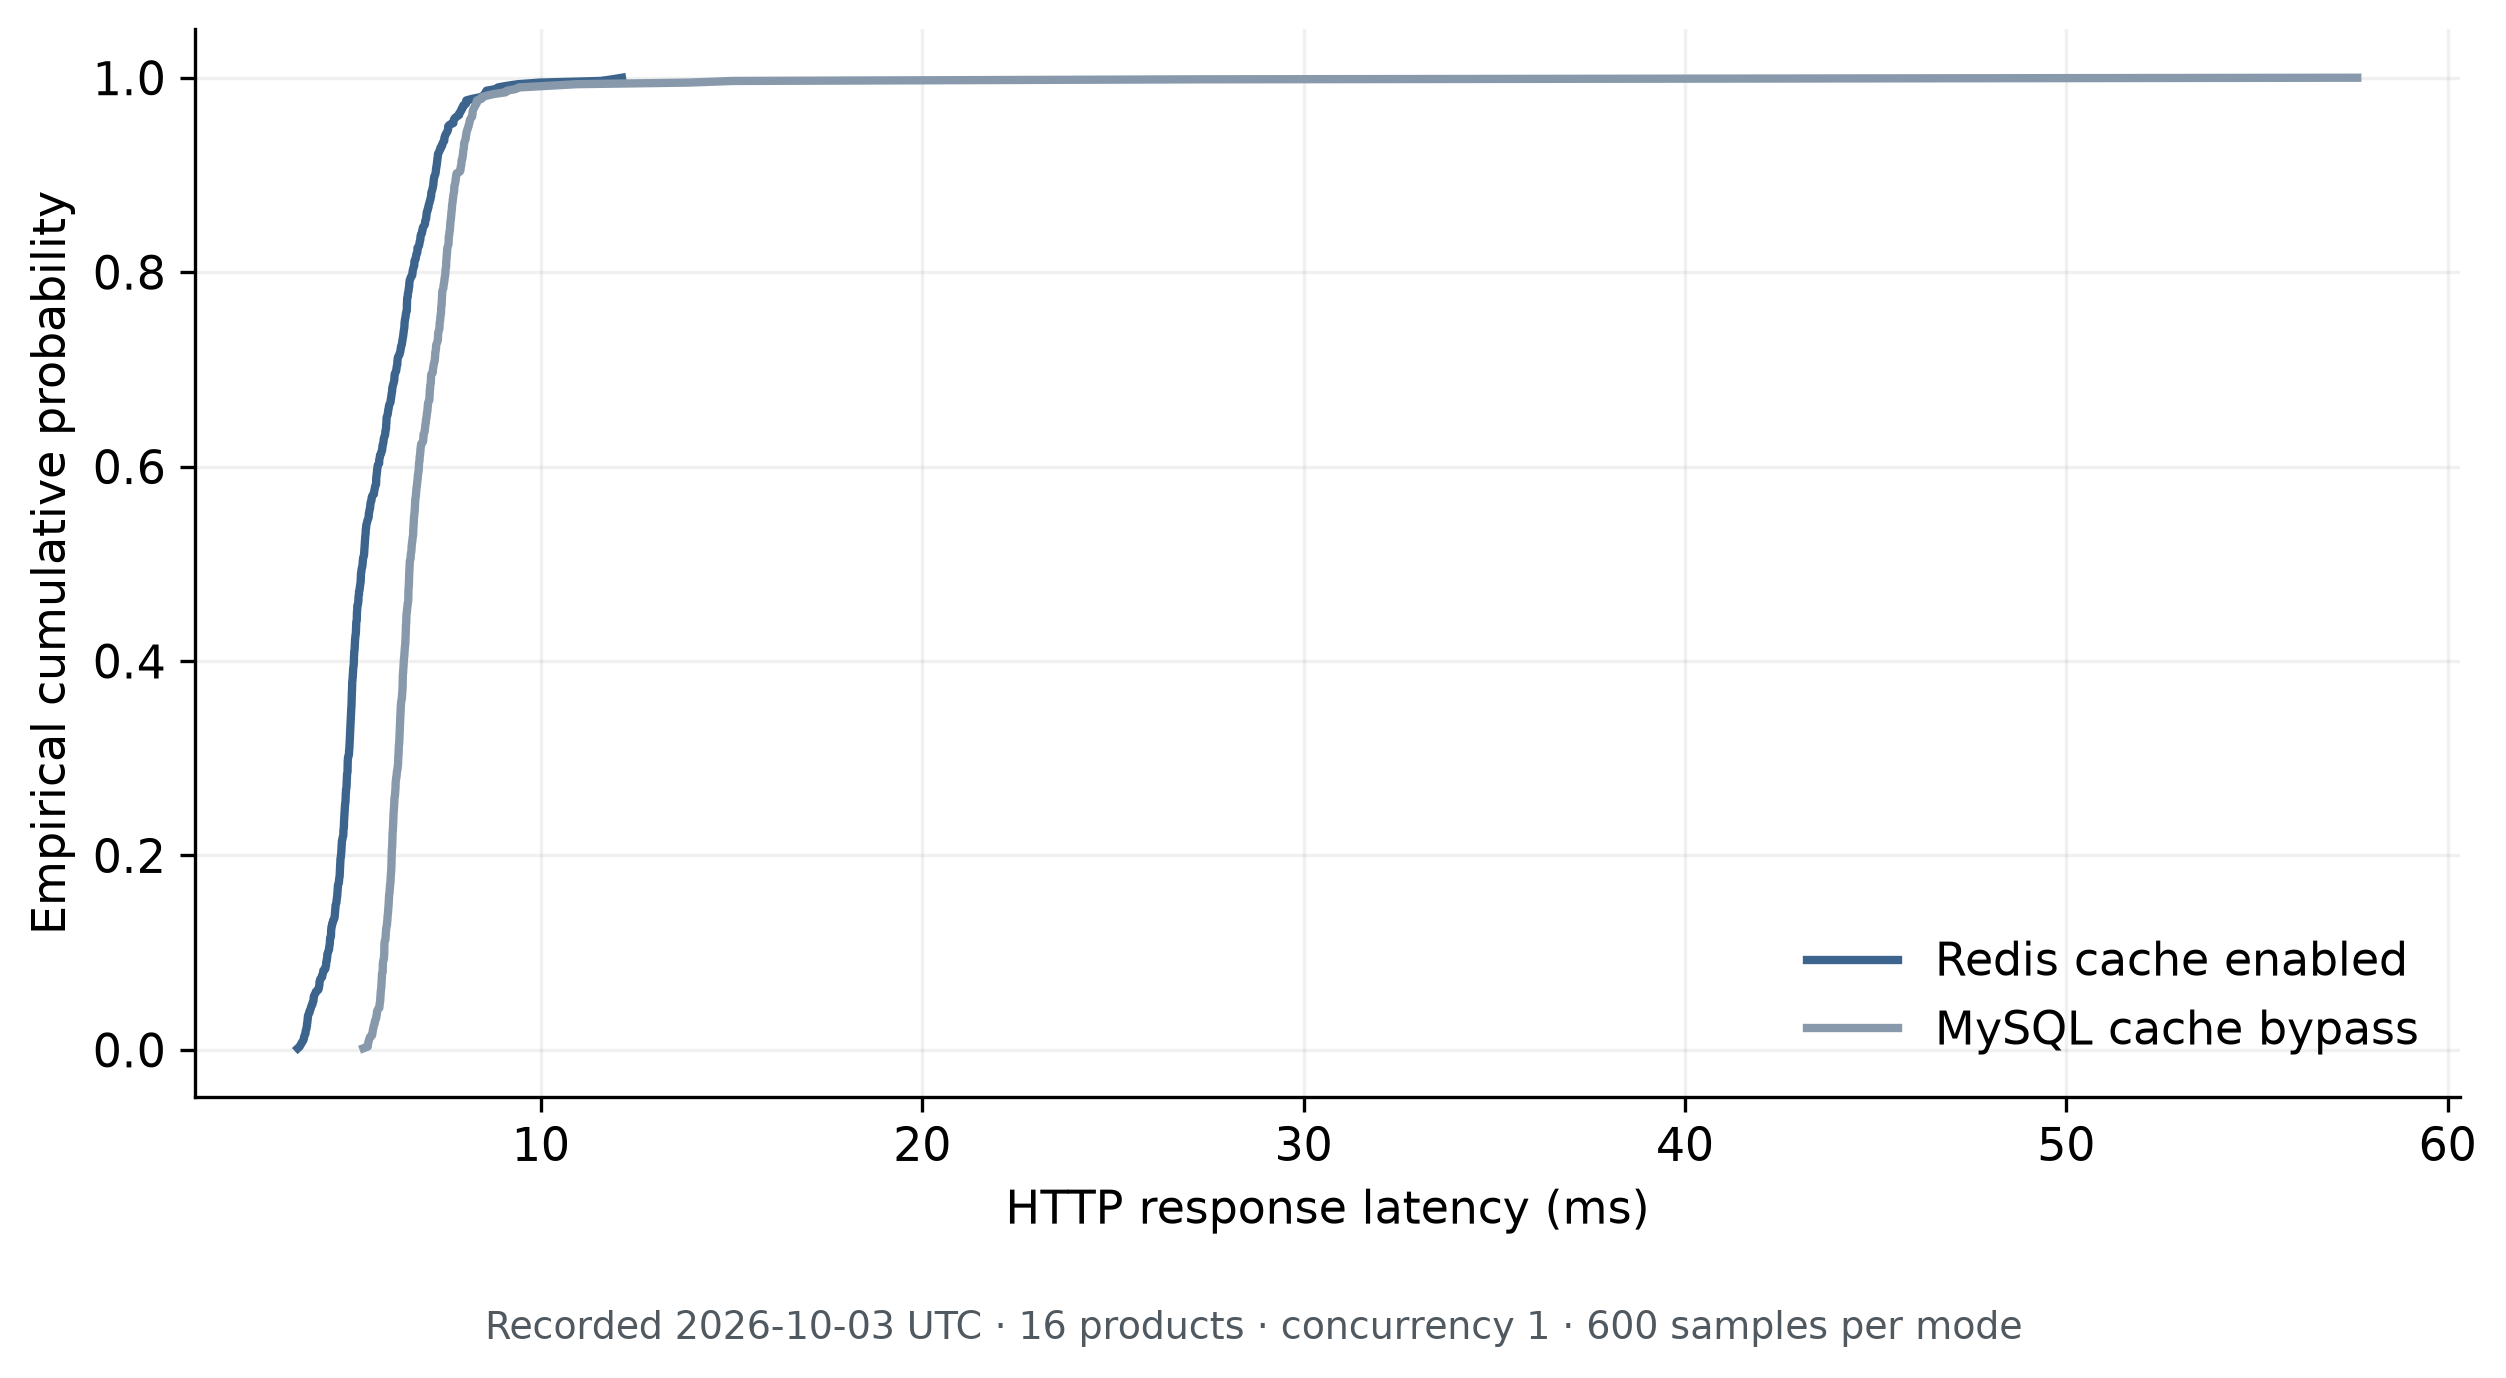
\includegraphics[width=\textwidth,height=0.40\textheight,keepaspectratio]{../figure-assets/evidence/05-latency-ecdf.png}
\caption{Empirical distribution of the preserved warning-query latencies}\label{fig:latency-ecdf}
\end{figure}

The box plot in Figure~\ref{fig:latency-box} shows variability and outlying observations. Those observations should not be silently removed merely to improve the visual result. They also should not be generalized into a production reliability rate. The sample is small in business scope and restricted to one read operation with sequential local traffic.


\begin{figure}[htbp]\centering
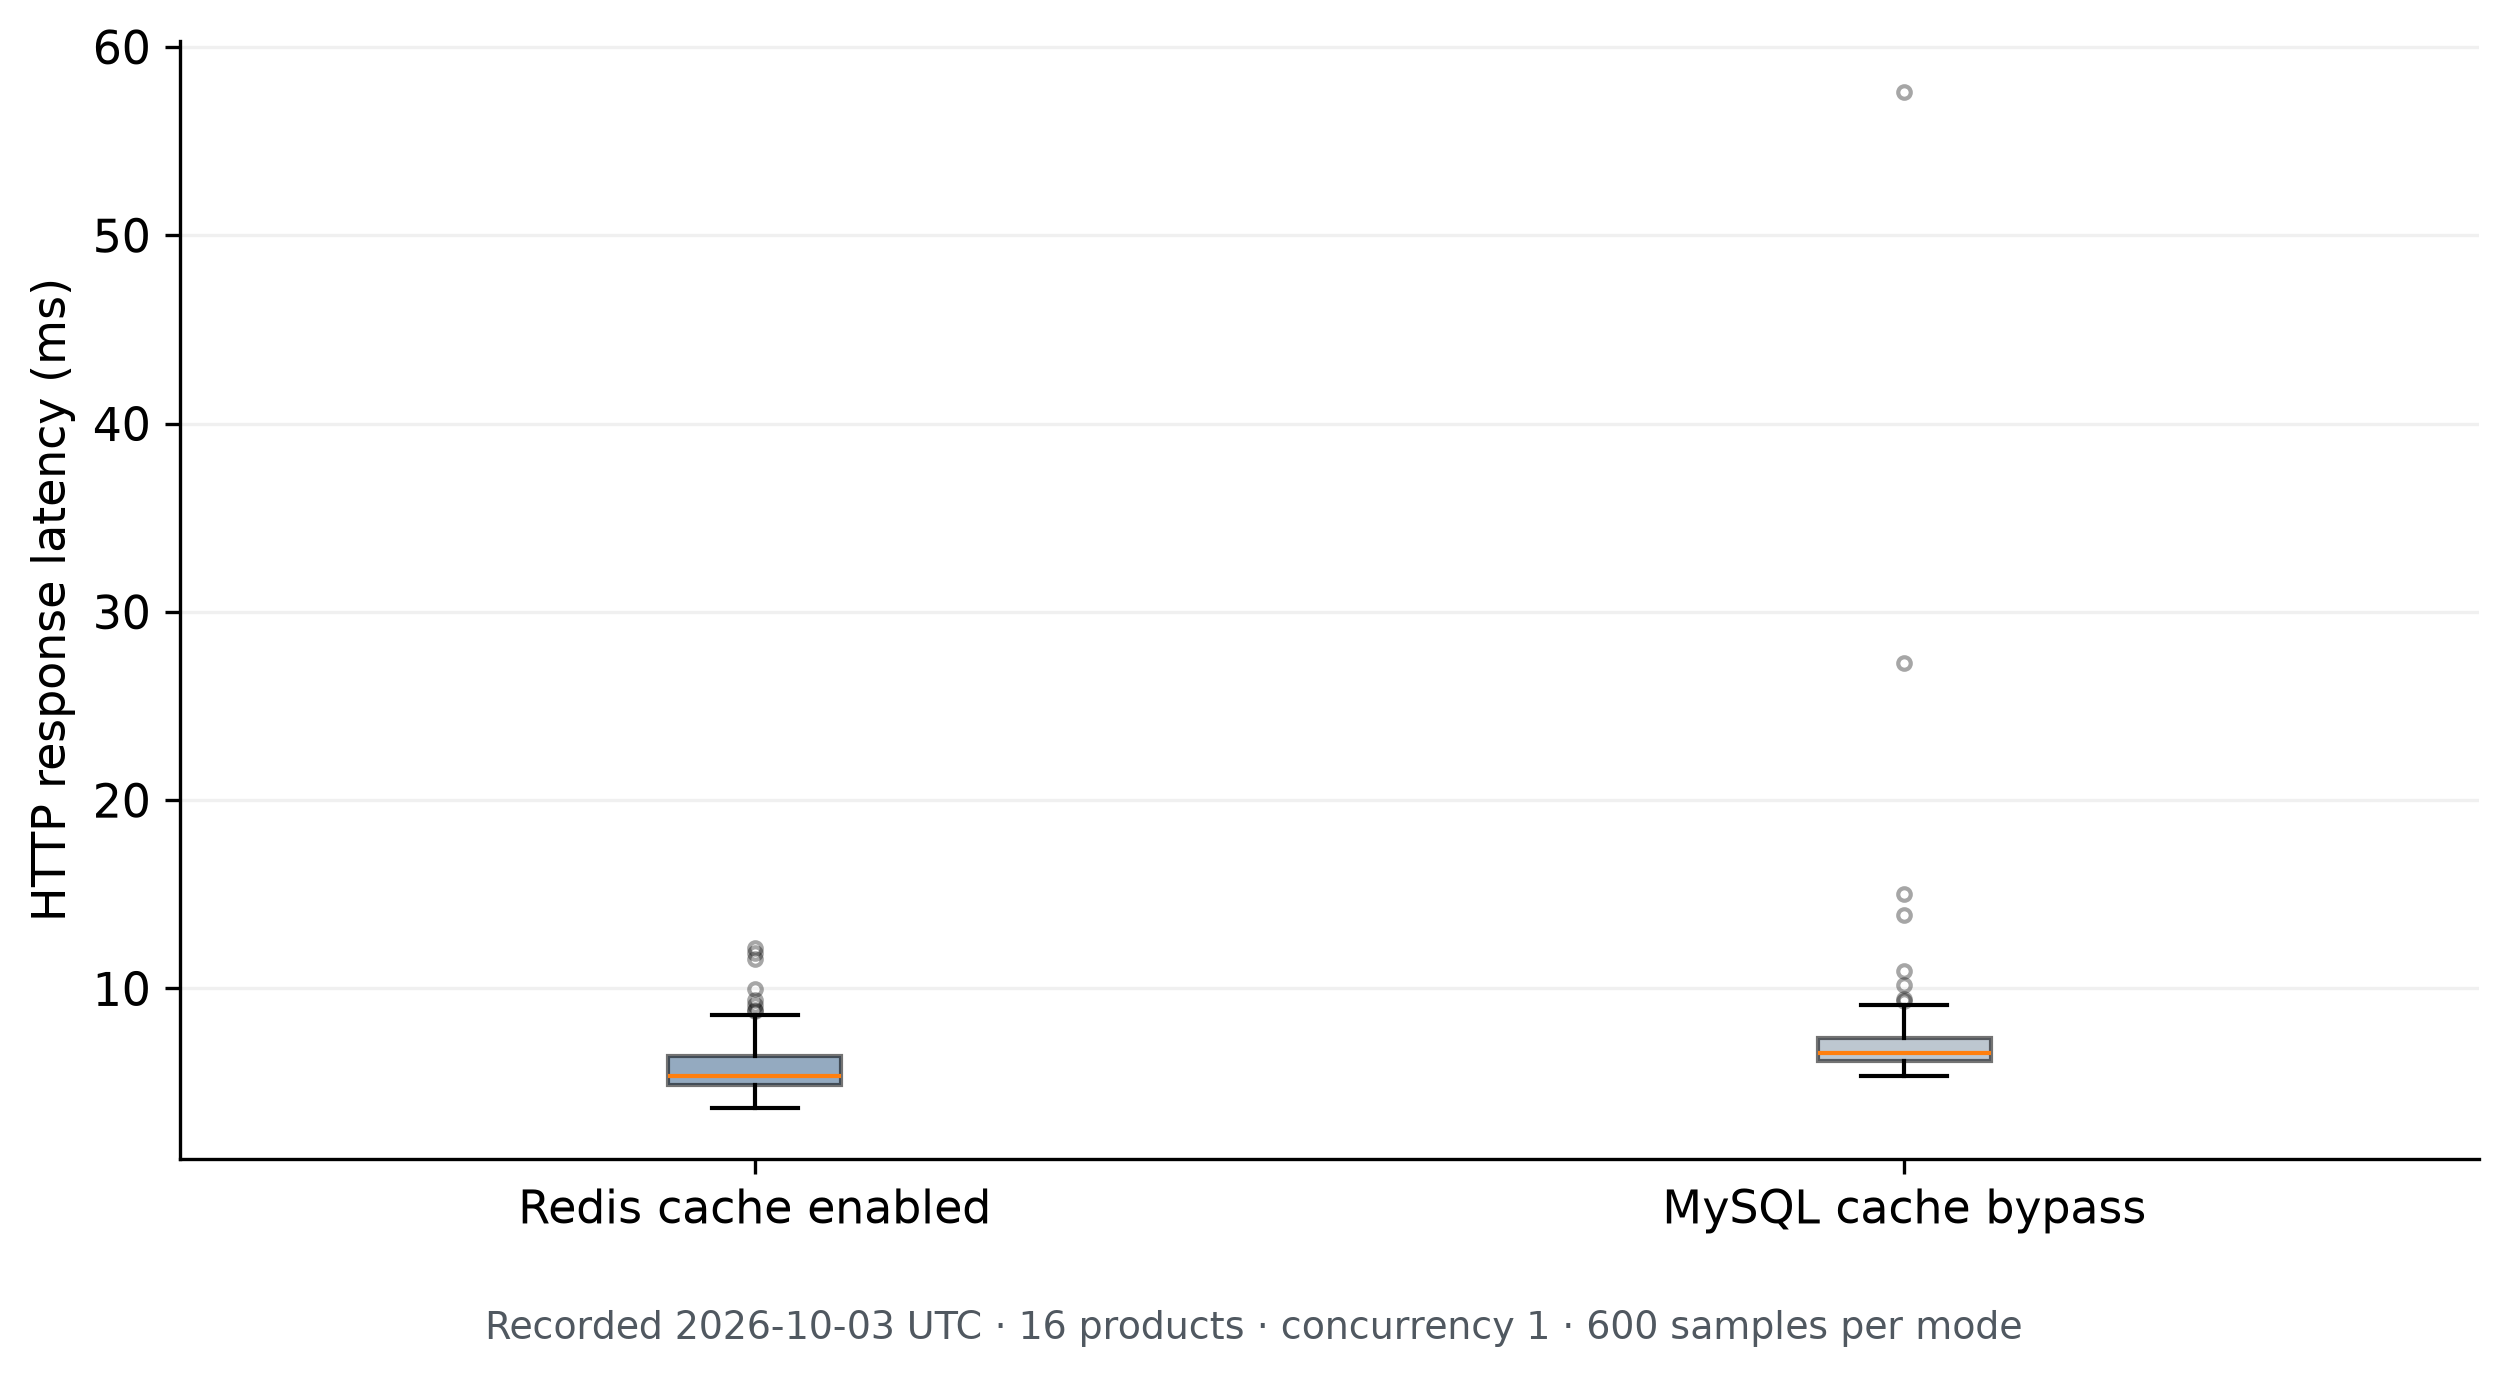
\includegraphics[width=\textwidth,height=0.40\textheight,keepaspectratio]{../figure-assets/evidence/06-latency-boxplot.png}
\caption{Local latency variability including observed outliers}\label{fig:latency-box}
\end{figure}

\FloatBarrier

\subsection{Interpretation and remaining performance work}

The cache reduces repeated page assembly in the tested workload, but each read still obtains a durable revision and checks session authority. A high cache-hit ratio is not equivalent to eliminating database access. The prototype's write path also advances a shared revision row. Testing many writers across different products is therefore a necessary next step before drawing conclusions about larger-store workload behavior.


Useful extensions would vary catalogue size, warning count, page size, concurrent readers and concurrent writers. They would report warm and cold cache behavior, latency distributions, rejected requests and database resource use. A production comparison should control relevant deployment variables and preserve raw samples. These proposed tests describe additional evaluation, not results already obtained.


\FloatBarrier

\section{Recorded failure and persistence checks}

The Redis recovery record stops and restarts only the cache service while MySQL remains available. A cache-enabled query during interruption is compared with the uncached baseline. The record reports the same database warning result during the outage and a recovered service afterward. Individual observed query times are approximately 10.49 ms before interruption, 12.25 ms while unavailable and 25.94 ms after recovery. They are individual observations, not estimates of a recovery-time distribution.


\begingroup\small\setstretch{1.05}\setlength{\tabcolsep}{3pt}\renewcommand{\arraystretch}{1.25}
\begin{longtable}{>{\raggedright\arraybackslash}p{0.3\textwidth}>{\raggedright\arraybackslash}p{0.3\textwidth}>{\raggedright\arraybackslash}p{0.3\textwidth}}
\caption{Recorded cache interruption and restart observations}\label{tab:recovery}\\
\toprule
\textbf{Observation} & \textbf{Recorded result} & \textbf{Supported interpretation} \\
\midrule\endfirsthead
\toprule
\textbf{Observation} & \textbf{Recorded result} & \textbf{Supported interpretation} \\
\midrule\endhead
\bottomrule\endfoot
Redis stopped with MySQL available & Same warning result & Cache outage did not remove authoritative warning data \\
Redis restarted & Recovered service and equivalent result & Normal cache service resumed in this check \\
Application restarted & Same selected stock and movement rows & Durable MySQL state survived ordinary process restart \\
Selected-row fingerprint & 34 rows and equal SHA-256 & Compared product and transaction data remained equal \\
\end{longtable}\endgroup

A separate persistence record compares selected product and transaction rows around an application restart using a fingerprint. It reports equality for thirty-four selected rows. This supports ordinary persistence of those records. It is not a backup restoration, disk-failure or full-database recovery test. Session survival is also a different property: the in-process login state may be lost while stock remains durable.


\FloatBarrier

\section{Traceability and validity of the conclusions}

The acceptance evidence is strongest where a requirement has a direct assertion. Non-negative concurrent stock has a final balance and a success-count check. Exact replay has an identifier and quantity check. Batch allocation has sellable-balance and remainder checks. Purchase approval has recheck, receipt and replay assertions. Acknowledgement and review have reviewer or snapshot checks. Weaker or absent evidence is identified separately, including sustained multi-user workload, external supplier integration and operational usability.


Internal validity is limited by the particular test scenarios and the execution environment. External validity is limited by demonstration data and the single-store boundary. Construct validity depends on using the intended metric: movement counts are not sales, current-price value is not profit, and response latency under one sequential query is not throughput capacity. The thesis maintains those distinctions throughout its figures and result tables.


The current evidence supports a working bounded inventory system with selected consistency and recovery properties. It does not establish a production SLA, a quantified reduction in supermarket stockouts or the safety of unrestricted public deployment. Those conclusions require additional operational controls, workloads and field observations beyond this development study.


\FloatBarrier

\section{Chapter summary}

Functional tests support the implemented stock arithmetic, audit path, role boundaries and selected warning transitions. Browser evidence supports the rendered workflow and selected operational journeys. The local cache benchmark reports a lower pooled median for the enabled path under a small sequential workload. Failure records support cache fallback and ordinary persistence. The following conclusion relates these findings to the original engineering questions and identifies the next work needed for a broader deployment.

\chapter*{CONCLUSION}\addcontentsline{toc}{chapter}{CONCLUSION}
The project produced a working single-store inventory and warning system with an auditable stock movement path. MySQL remains the source of truth, while Redis is an optional read accelerator. Tests support non-negative stock under the selected concurrency cases, exact retry behavior, role boundaries, warning lifecycle transitions, and database fallback during Redis failure. The results do not establish a production SLA, business benefit, or real-store usability outcome. Whole-unit stock, manual thresholds, single-node sessions, and the absence of a field study remain important limits.

The next work should validate the workflow with store staff, add the domain controls required for batches and fractional units, test backup restoration and security hardening, and evaluate a point-of-sale integration. Automatic purchasing and forecasting should be considered only after demand and supplier data are available.
\bibliographystyle{plainnat}\bibliography{references}
\end{document}
